\documentclass{article}
\usepackage{graphicx,caption}
\usepackage{enumitem}
\usepackage{epstopdf,subcaption}
\usepackage{psfrag}
\usepackage{amsmath,amssymb,epsf}
\usepackage{verbatim}
\usepackage[hyphens]{url}
\usepackage{amsmath}
\usepackage{color}
\usepackage{bbm}
\usepackage{listings}
\usepackage{setspace}
\usepackage{float}
\definecolor{Code}{rgb}{0,0,0}
\definecolor{Decorators}{rgb}{0.5,0.5,0.5}
\definecolor{Numbers}{rgb}{0.5,0,0}
\definecolor{MatchingBrackets}{rgb}{0.25,0.5,0.5}
\definecolor{Keywords}{rgb}{0,0,1}
\definecolor{self}{rgb}{0,0,0}
\definecolor{Strings}{rgb}{0,0.63,0}
\definecolor{Comments}{rgb}{0,0.63,1}
\definecolor{Backquotes}{rgb}{0,0,0}
\definecolor{Classname}{rgb}{0,0,0}
\definecolor{FunctionName}{rgb}{0,0,0}
\definecolor{Operators}{rgb}{0,0,0}
\definecolor{Background}{rgb}{0.98,0.98,0.98}
\lstdefinelanguage{Python}{
numbers=left,
numberstyle=\footnotesize,
numbersep=1em,
xleftmargin=1em,
framextopmargin=2em,
framexbottommargin=2em,
showspaces=false,
showtabs=false,
showstringspaces=false,
frame=l,
tabsize=4,
% Basic
basicstyle=\ttfamily\footnotesize\setstretch{1},
backgroundcolor=\color{Background},
% Comments
commentstyle=\color{Comments}\slshape,
% Strings
stringstyle=\color{Strings},
morecomment=[s][\color{Strings}]{"""}{"""},
morecomment=[s][\color{Strings}]{'''}{'''},
% keywords
morekeywords={import,from,class,def,for,while,if,is,in,elif,else,not,and,or
,print,break,continue,return,True,False,None,access,as,,del,except,exec
,finally,global,import,lambda,pass,print,raise,try,assert},
keywordstyle={\color{Keywords}\bfseries},
% additional keywords
morekeywords={[2]@invariant},
keywordstyle={[2]\color{Decorators}\slshape},
emph={self},
emphstyle={\color{self}\slshape},
%
}

%%% Change the following flag to toggle between questions or solutions
\def\solutions{1}

\pagestyle{empty} \addtolength{\textwidth}{1.0in}
\addtolength{\textheight}{0.5in}
\addtolength{\oddsidemargin}{-0.5in}
\addtolength{\evensidemargin}{-0.5in}
\newcommand{\ruleskip}{\bigskip\hrule\bigskip}
\newcommand{\nodify}[1]{{\sc #1}}
\newcommand{\points}[1]{{\textbf{[#1 points]}}}
\newcommand{\subquestionpoints}[1]{{[#1 points]}}
\newcommand{\xsi}{x^{(i)}}
\newcommand{\zsi}{z^{(i)}}
\newenvironment{answer}{{\bf Answer:} \sf \begingroup\color{red}}{\endgroup}%

\newcommand{\bitem}{\begin{list}{$\bullet$}%
{\setlength{\itemsep}{0pt}\setlength{\topsep}{0pt}%
\setlength{\rightmargin}{0pt}}}
\newcommand{\eitem}{\end{list}}

\setlength{\parindent}{0pt} \setlength{\parskip}{0.5ex}
\setlength{\unitlength}{1cm}

\renewcommand{\Re}{{\mathbb R}}
\newcommand{\R}{\mathbb{R}}
\newcommand{\what}[1]{\widehat{#1}}

\renewcommand{\comment}[1]{}
\newcommand{\mc}[1]{\mathcal{#1}}
\newcommand{\half}{\frac{1}{2}}
\newcommand{\KL}{D_{\text{KL}}}

\begin{document}

\pagestyle{myheadings} \markboth{}{CS229 Problem Set \#3}

\ifnum\solutions=1 {
{\huge\noindent CS 229, Fall 2018\\
Problem Set \#3 Solutions: Deep Learning \& Unsupervised learning}\\\\
YOUR NAME HERE (\texttt{YOUR SUNET HERE})
} \else {\huge
\noindent CS 229, Fall 2018\\
Problem Set \#3: Deep Learning \& Unsupervised learning
} \fi

\ruleskip

{\bf Due Wednesday, Nov 14 at 11:59 pm on Gradescope.}

\medskip

\clearpage
\item \points{40} {\bf Linear Classifiers (logistic regression and GDA)}

In this problem, we cover two probabilistic linear classifiers we have
covered in class so far. First, a discriminative linear classifier: logistic
regression. Second, a generative linear classifier: Gaussian discriminant
analysis (GDA). Both the algorithms find a linear decision boundary that
separates the data into two classes, but make different assumptions. Our goal
in this problem is to get a deeper understanding of the similarities and
differences (and, strengths and weaknesses) of these two algorithms.

For this problem, we will consider two datasets, provided in the following
files:
\begin{enumerate}[label=\roman*.]
	\item \url{data/ds1_{train,valid}.csv}
	\item \url{data/ds2_{train,valid}.csv}
\end{enumerate}
Each file contains $m$ examples, one example $(x^{(i)}, y^{(i)})$ per row.
In particular, the $i$-th row contains columns $x^{(i)}_0\in\Re$,
$x^{(i)}_1\in\Re$, and $y^{(i)}\in\{0, 1\}$. In the subproblems that follow, we
will investigate using logistic regression and Gaussian discriminant analysis
(GDA) to perform binary classification on these two datasets.

\begin{enumerate}
	\item \subquestionpoints{10}
In lecture we saw the average empirical loss for logistic regression:
\begin{equation*}
	J(\theta)
	= -\frac{1}{m} \sum_{i=1}^m y^{(i)}\log(h_{\theta}(x^{(i)}))
		+  (1 - y^{(i)})\log(1 - h_{\theta}(x^{(i)})),
\end{equation*}
where $y^{(i)} \in \{0, 1\}$, $h_\theta(x) = g(\theta^T x)$ and
$g(z) = 1 / (1 + e^{-z})$.

Find the Hessian $H$ of this function, and show that for any vector $z$, it
holds true that
%
\begin{equation*}
    z^T H z \ge 0.
\end{equation*}
%
{\bf Hint:} You may want to start by showing that
$\sum_i\sum_j z_i x_i x_j z_j = (x^Tz)^2 \geq 0$. Recall also that
$g'(z) = g(z)(1-g(z))$.

{\bf Remark:} This is one of the standard ways of showing that the matrix $H$
is positive semi-definite, written ``$H \succeq 0$.''  This implies that $J$ is
convex, and has no local minima other than the global one. If you have some
other way of showing $H \succeq 0$, you're also welcome to use your method
instead of the one above.

\ifnum\solutions=1 {
  \begin{answer}
Throughout the problem set $(a,b)$ denoted the inner(dot) product of the vectors $a,b.$
It is easy to see that for the logistic function $g(z)$, we have $g'(z)= g(z)(1- g(z)).$ We use this to calculate the partial derivative of the loss functions. 
$$\frac{\partial h_{\theta}(x)}{\partial \theta_i} = \frac{\partial g(\theta^Tx)}{\partial \theta_i} = g(\theta^Tx) (1 - g(\theta^Tx))
\frac{\partial}{\partial\theta_i}(\theta^Tx) = h_{\theta}(x) (1 - h_{\theta}(x)) x_i$$
Hence,

$$\frac{\partial log(h_{\theta}(x))}{\partial \theta_i} = \frac{h'_{\theta}(x)}{h_{\theta}(x)} = (1 - h_{\theta}(x))x_i.$$
Similarly,

$$\frac{\partial (1 - log(1 - h_{\theta}(x)))}{\partial \theta_i} = - \frac{h'_{\theta}(x)}{1 - h_{\theta}(x)} = -h_{\theta}(x)x_i.$$

Using the above computations and some simplification we obtain the partial derivative of the loss function wrt $i-$th component.
$$\frac{\partial J(\theta)}{\partial \theta_i} = - \frac{1}{m}\sum_{k = 1}^{m }x_i^{(k)}( y^{(k)} - h_{\theta}(x^{(k)})). \eqno(1)$$

Note that the above sum can conveniently be expressed in the form of inner product and we will use such form in the coding part using numpy's dot operation.

The formula (1)  allow us to easily find the entries of the Hessian.

$$\frac{\partial^2 J(\theta)}{\partial \theta_i \partial\theta_j} = 
\frac{1}{m}\sum_{k = 0}^{m - 1}g'(\theta^Tx^{(k)}))x_i^{(k)}x_j^{(k)}. \eqno(2)$$
Thus, the $(i,j)-$ th entry  of the Hessian matrix is given by the right hand side of (2).
Now we show that the Hessian is positive semi-definite. Below $(a,b)$ denotes the inner product of $a$ and $b.$
$$z^THz = (Hz,z)=  \sum_{i,j}\sum_{k = 1}^{m}g'(\theta^Tx^{(k)})x_i^{(k)}x_j^{(k)}z_iz_j=  \sum_{k = 1}^m\sum_{i,j}g'(\theta^Tx^{(k)})x_i^{(k)}x_j^{(k)}z_iz_j$$
$$= \sum_{k = 1}^m g'(\theta^Tx^{(k)}) (x^Tz)^2 \ge 0.$$
as the logistic function is non -decreasing so its derivative is non-negative (or $g' = g(1-g)\ge 0$).

\end{answer}

  
} \fi

	\clearpage
\item \subquestionpoints{5} \textbf{Coding problem.}
Follow the instructions in \texttt{src/p01b\_logreg.py} to train a
logistic regression classifier using Newton's Method.
Starting with $\theta = \vec{0}$, run Newton's Method until the updates to
$\theta$ are small: Specifically,  train until the first iteration $k$ such
that $\|\theta_{k} - \theta_{k-1}\|_1 < \epsilon$, where
$\epsilon = 1\times 10^{-5}$. Make sure to write your model's predictions to
the file specified in the code.

\ifnum\solutions=1 {
  \begin{answer}
Done!
\end{answer}

} \fi

	\clearpage
\item \subquestionpoints{5}
Recall that in GDA we model the joint distribution of $(x, y)$ by the following
equations:
%
\begin{eqnarray*}
	p(y) &=& \begin{cases}
	\phi & \mbox{if~} y = 1 \\
	1 - \phi & \mbox{if~} y = 0 \end{cases} \\
	p(x | y=0) &=& \frac{1}{(2\pi)^{n/2} |\Sigma|^{1/2}}
		\exp\left(-\frac{1}{2}(x-\mu_{0})^T \Sigma^{-1} (x-\mu_{0})\right) \\
	p(x | y=1) &=& \frac{1}{(2\pi)^{n/2} |\Sigma|^{1/2}}
		\exp\left(-\frac{1}{2}(x-\mu_1)^T \Sigma^{-1} (x-\mu_1) \right),
\end{eqnarray*}
%
where $\phi$, $\mu_0$, $\mu_1$, and $\Sigma$ are the parameters of our model.

Suppose we have already fit $\phi$, $\mu_0$, $\mu_1$, and $\Sigma$, and now
want to predict $y$ given a new point $x$. To show that GDA results in a
classifier that has a linear decision boundary, show the posterior distribution
can be written as
%
\begin{equation*}
	p(y = 1\mid x; \phi, \mu_0, \mu_1, \Sigma)
	= \frac{1}{1 + \exp(-(\theta^T x + \theta_0))},
\end{equation*}
%
where $\theta\in\Re^n$ and $\theta_{0}\in\Re$ are appropriate functions of
$\phi$, $\Sigma$, $\mu_0$, and $\mu_1$.

\ifnum\solutions=1{
  \begin{answer}
Apply Bayes
$$p(y = 1| x) = \frac{p(x| y=1)p(y = 1)}{p(x| y=1)p(y = 1) + p(x| y=0)p(y = 0)} = \frac{1}{1 + \frac{p(x| y=0)p(y = 0)}{p(x| y=1)p(y = 1)}}.$$
Note that $\frac{p(y = 0)}{p(y = 1)} = exp(ln(\frac{1-\phi}{\phi})$
For simplicity  denote A = $\Sigma^{-1}.$
Note that
$$\frac{p(x| y=0)}{p(x| y=1)} = exp(-\frac{1}{2}(A(x- \mu_0), x - \mu_0) - (A(x- \mu_1), x - \mu_1))) $$$$= exp(-\frac 12((Ax,x) - 2(Ax, \mu_0) + (\mu_0, \mu_0) - (Ax,x) + 2(Ax, \mu_1) + (\mu_1, \mu_1)))$$
$$= exp(-( -(Ax, \mu_0) + \frac 12(A\mu_0, \mu_0) + (Ax, \mu_1) - \frac12(A\mu_1, \mu_1))) = exp(-(\mu_1 - \mu_0)^TAx + \frac{1}{2}((A\mu_0,\mu_0) - (A\mu_1,\mu_1)).$$
From this we find $\theta^T = (\mu_1 - \mu_0)^TA$ hence 
$$\theta = (\Sigma^{-1})^T(\mu_1 - \mu_0)$$
and
$$\theta_0 = \frac{1}{2}((\Sigma^{-1}\mu_0,\mu_0) - (\Sigma^{-1}\mu_1,\mu_1)) - ln(\frac{1-\phi}{\phi}).$$

\end{answer}

}\fi

	\clearpage
\item \subquestionpoints{7} For this part of the problem only, you may
  assume $n$ (the dimension of $x$) is 1, so that $\Sigma = [\sigma^2]$ is
  just a real number, and likewise the determinant of $\Sigma$ is given by
  $|\Sigma| = \sigma^2$.  Given the dataset, we claim that the maximum
  likelihood estimates of the parameters are given by
  \begin{eqnarray*}
    \phi &=& \frac{1}{m} \sum_{i=1}^m 1\{y^{(i)} = 1\} \\
\mu_{0} &=& \frac{\sum_{i=1}^m 1\{y^{(i)} = {0}\} x^{(i)}}{\sum_{i=1}^m
1\{y^{(i)} = {0}\}} \\
\mu_1 &=& \frac{\sum_{i=1}^m 1\{y^{(i)} = 1\} x^{(i)}}{\sum_{i=1}^m 1\{y^{(i)}
= 1\}} \\
\Sigma &=& \frac{1}{m} \sum_{i=1}^m (x^{(i)} - \mu_{y^{(i)}}) (x^{(i)} -
\mu_{y^{(i)}})^T
  \end{eqnarray*}
  The log-likelihood of the data is
  \begin{eqnarray*}
\ell(\phi, \mu_{0}, \mu_1, \Sigma) &=& \log \prod_{i=1}^m p(x^{(i)} , y^{(i)};
\phi, \mu_{0}, \mu_1, \Sigma) \\
&=& \log \prod_{i=1}^m p(x^{(i)} | y^{(i)}; \mu_{0}, \mu_1, \Sigma) p(y^{(i)};
\phi).
  \end{eqnarray*}
By maximizing $\ell$ with respect to the four parameters,
prove that the maximum likelihood estimates of $\phi$, $\mu_{0}, \mu_1$, and
$\Sigma$ are indeed as given in the formulas above.  (You may assume that there
is at least one positive and one negative example, so that the denominators in
the definitions of $\mu_{0}$ and $\mu_1$ above are non-zero.)

\ifnum\solutions=1 {
  \begin{answer}
The product and the sums run from  1 to m, so for simplicity I drop the limits. Note that
$$l = \log\prod p(y^{(i)}| x^{(i)})p(y{(i)}) = \sum\log p(y^{(i)}| x^{(i)})p(y{(i)}) = $$$$
 -m\log(\sigma) + c_0 - \sum\big( y^{(i)}\frac{(x^{(i)} - \mu_0)^2}{2\sigma^2} + (1- y^{(i)})\frac{(x^{(i)} - \mu_1)^2}{2\sigma^2}\big) + \sum(y^{(i)}\phi + (1-y^{(i)})(1-\phi)).$$
 
 Now we calculate the partial derivatives.
 
 $$\frac{\partial}{\partial\phi} = \sum(\frac{y^{(i)}}{\phi} + \frac{1- y^{(i)}}{1-\phi}) = 0.$$
 The numerator after the sum is then $\sum y^{(i)} - m\phi$ and so
 $$\phi= \frac{\sum y^{(i)}}{m}.$$
 Not that the formula is exactly as the formula given in the problem because if $y^{(i)} = 0$ the $i-$th term of the sum is $0.$ Hence this formula can be represented with the characteristic function. I will not be re-writing this as well as the problems below as I do not know how useful it may be in the coding part.
 Further derivatives (enough to show $\mu_0$):
 $$\frac{\partial l}{\partial\mu_0} =\sum\frac{y^{(i)}(x^{(i)} - \mu_0 )}{\sigma^2} = \frac{\sum x^{(i)}y^{(i)} - \mu_0\sum y^{(i)}}{\sigma^2}.$$
 Hence we obtain
 $$\mu_0 = \frac{\sum x^{(i)}y^{(i)}}{\sum y^{(i)}}.$$
 Finally, 
 $$\frac{\partial l}{\partial \sigma} = \frac{m}{\sigma} - \frac{1}{\sigma^3}(\sum\big( y^{(i)}\frac{(x^{(i)} - \mu_0)^2}{2\sigma^2} + (1- y^{(i)})\frac{(x^{(i)} - \mu_1)^2}{2\sigma^2}\big)).$$
 By solving this equation for $\sigma$ we obtain the desired result.
 
 
 
\end{answer}

} \fi

	\clearpage
\item \subquestionpoints{3} \textbf{Coding problem.}
In \texttt{src/p01e\_gda.py}, fill in the code to
calculate $\phi$, $\mu_{0}$, $\mu_{1}$, and $\Sigma$, use these parameters
to derive $\theta$, and use the resulting GDA model to make predictions on the
validation set.

\ifnum\solutions=1 {
  \begin{answer}
\end{answer}

} \fi

	\clearpage
\item \subquestionpoints{5}
For Dataset 1, create a plot of the validation set with $x_1$ on the horizontal
axis, and $x_2$ on the vertical axis. To visualize the two classes, use a
different symbol for examples $x^{(i)}$ with $y^{(i)} = 0$ than for those with
$y^{(i)} = 1$. On the same figure, plot the decision boundary found by logistic
regression in part (b). Make an identical plot with the decision boundary found
by GDA in part (e).

\ifnum\solutions=1 {
  
\begin{answer}
\begin{figure}[htbp]
    \begin{subfigure}[b]{0.5\linewidth}
        \centering
        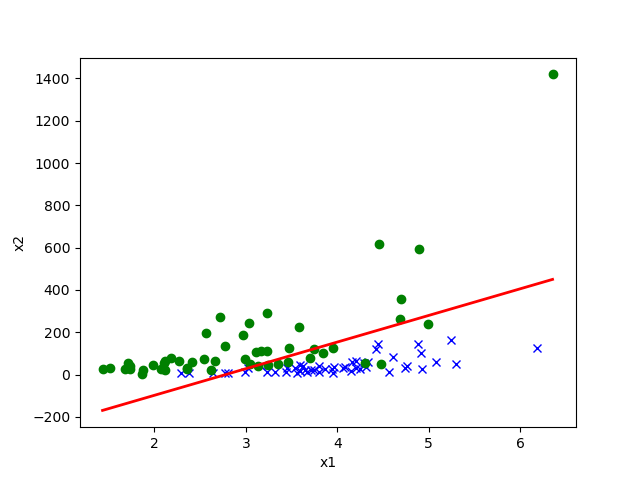
\includegraphics[width=\linewidth]{p01b_pred_1_txt.png}
        \subcaption{Logistic Regression for Dataset 1}
    \end{subfigure}
    \begin{subfigure}[b]{0.5\linewidth}
        \centering
        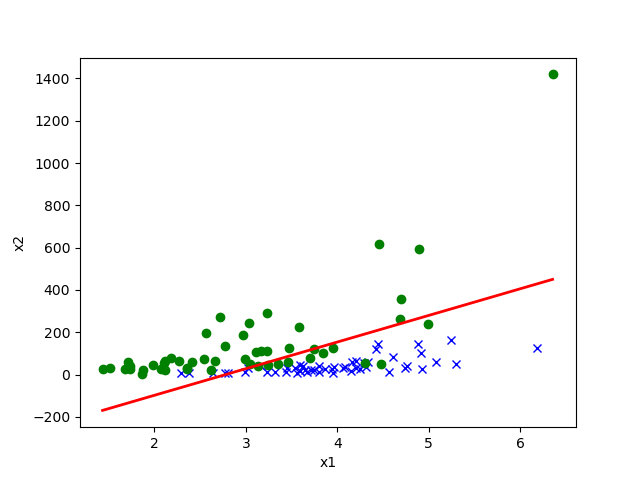
\includegraphics[width=\linewidth]{p01e_pred_1_txt.png}
        \subcaption{GDA for Dataset 1}
    \end{subfigure}

\end{figure}

\end{answer}
} \fi

	\clearpage
\item \subquestionpoints{5}
Repeat the steps in part (f) for Dataset 2. On which dataset does GDA seem to
perform worse than logistic regression? Why might this be the case?

\ifnum\solutions=1{
  \begin{answer}
\begin{figure}[htbp]
    \begin{subfigure}[b]{0.5\linewidth}
        \centering
        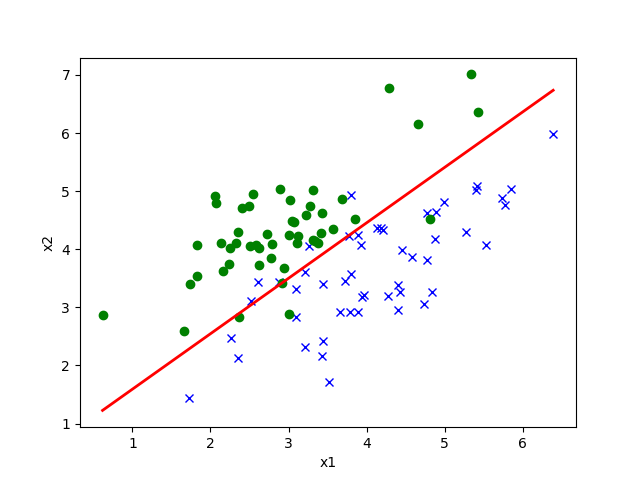
\includegraphics[width=\linewidth]{output/p01b_pred_2.txt.png}
        \subcaption{Logistic Regression for Dataset 2}
    \end{subfigure}
    \begin{subfigure}[b]{0.5\linewidth}
        \centering
        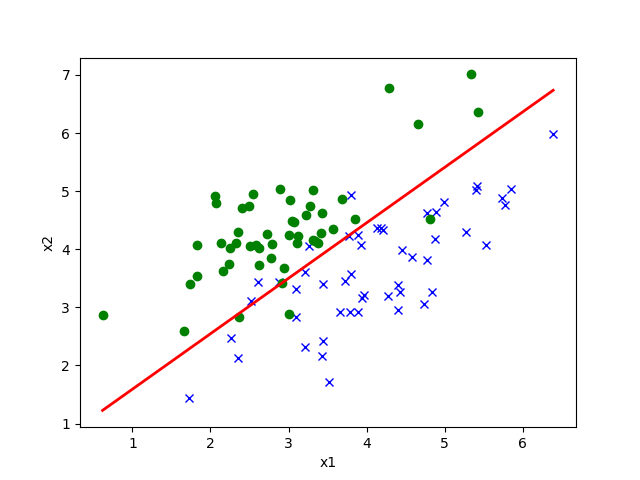
\includegraphics[width=\linewidth]{output/p01e_pred_2.txt.png}
        \subcaption{GDA for Dataset 2}
    \end{subfigure}

\end{figure}
\end{answer}

}\fi

	\clearpage
\item \points{3 extra credit} For the dataset where GDA performed worse in
parts (f) and (g), can you find a transformation of the $x^{(i)}$'s such
that GDA performs significantly better? What is this transformation?

\ifnum\solutions=1{
  \begin{answer}
\end{answer}

}\fi

\end{enumerate}


\begin{enumerate}[wide, labelwidth=!, labelindent=0pt]

\clearpage
\item \points{40} {\bf Linear Classifiers (logistic regression and GDA)}

In this problem, we cover two probabilistic linear classifiers we have
covered in class so far. First, a discriminative linear classifier: logistic
regression. Second, a generative linear classifier: Gaussian discriminant
analysis (GDA). Both the algorithms find a linear decision boundary that
separates the data into two classes, but make different assumptions. Our goal
in this problem is to get a deeper understanding of the similarities and
differences (and, strengths and weaknesses) of these two algorithms.

For this problem, we will consider two datasets, provided in the following
files:
\begin{enumerate}[label=\roman*.]
	\item \url{data/ds1_{train,valid}.csv}
	\item \url{data/ds2_{train,valid}.csv}
\end{enumerate}
Each file contains $m$ examples, one example $(x^{(i)}, y^{(i)})$ per row.
In particular, the $i$-th row contains columns $x^{(i)}_0\in\Re$,
$x^{(i)}_1\in\Re$, and $y^{(i)}\in\{0, 1\}$. In the subproblems that follow, we
will investigate using logistic regression and Gaussian discriminant analysis
(GDA) to perform binary classification on these two datasets.

\begin{enumerate}
	\item \subquestionpoints{10}
In lecture we saw the average empirical loss for logistic regression:
\begin{equation*}
	J(\theta)
	= -\frac{1}{m} \sum_{i=1}^m y^{(i)}\log(h_{\theta}(x^{(i)}))
		+  (1 - y^{(i)})\log(1 - h_{\theta}(x^{(i)})),
\end{equation*}
where $y^{(i)} \in \{0, 1\}$, $h_\theta(x) = g(\theta^T x)$ and
$g(z) = 1 / (1 + e^{-z})$.

Find the Hessian $H$ of this function, and show that for any vector $z$, it
holds true that
%
\begin{equation*}
    z^T H z \ge 0.
\end{equation*}
%
{\bf Hint:} You may want to start by showing that
$\sum_i\sum_j z_i x_i x_j z_j = (x^Tz)^2 \geq 0$. Recall also that
$g'(z) = g(z)(1-g(z))$.

{\bf Remark:} This is one of the standard ways of showing that the matrix $H$
is positive semi-definite, written ``$H \succeq 0$.''  This implies that $J$ is
convex, and has no local minima other than the global one. If you have some
other way of showing $H \succeq 0$, you're also welcome to use your method
instead of the one above.

\ifnum\solutions=1 {
  \begin{answer}
Throughout the problem set $(a,b)$ denoted the inner(dot) product of the vectors $a,b.$
It is easy to see that for the logistic function $g(z)$, we have $g'(z)= g(z)(1- g(z)).$ We use this to calculate the partial derivative of the loss functions. 
$$\frac{\partial h_{\theta}(x)}{\partial \theta_i} = \frac{\partial g(\theta^Tx)}{\partial \theta_i} = g(\theta^Tx) (1 - g(\theta^Tx))
\frac{\partial}{\partial\theta_i}(\theta^Tx) = h_{\theta}(x) (1 - h_{\theta}(x)) x_i$$
Hence,

$$\frac{\partial log(h_{\theta}(x))}{\partial \theta_i} = \frac{h'_{\theta}(x)}{h_{\theta}(x)} = (1 - h_{\theta}(x))x_i.$$
Similarly,

$$\frac{\partial (1 - log(1 - h_{\theta}(x)))}{\partial \theta_i} = - \frac{h'_{\theta}(x)}{1 - h_{\theta}(x)} = -h_{\theta}(x)x_i.$$

Using the above computations and some simplification we obtain the partial derivative of the loss function wrt $i-$th component.
$$\frac{\partial J(\theta)}{\partial \theta_i} = - \frac{1}{m}\sum_{k = 1}^{m }x_i^{(k)}( y^{(k)} - h_{\theta}(x^{(k)})). \eqno(1)$$

Note that the above sum can conveniently be expressed in the form of inner product and we will use such form in the coding part using numpy's dot operation.

The formula (1)  allow us to easily find the entries of the Hessian.

$$\frac{\partial^2 J(\theta)}{\partial \theta_i \partial\theta_j} = 
\frac{1}{m}\sum_{k = 0}^{m - 1}g'(\theta^Tx^{(k)}))x_i^{(k)}x_j^{(k)}. \eqno(2)$$
Thus, the $(i,j)-$ th entry  of the Hessian matrix is given by the right hand side of (2).
Now we show that the Hessian is positive semi-definite. Below $(a,b)$ denotes the inner product of $a$ and $b.$
$$z^THz = (Hz,z)=  \sum_{i,j}\sum_{k = 1}^{m}g'(\theta^Tx^{(k)})x_i^{(k)}x_j^{(k)}z_iz_j=  \sum_{k = 1}^m\sum_{i,j}g'(\theta^Tx^{(k)})x_i^{(k)}x_j^{(k)}z_iz_j$$
$$= \sum_{k = 1}^m g'(\theta^Tx^{(k)}) (x^Tz)^2 \ge 0.$$
as the logistic function is non -decreasing so its derivative is non-negative (or $g' = g(1-g)\ge 0$).

\end{answer}

  
} \fi

	\clearpage
\item \subquestionpoints{5} \textbf{Coding problem.}
Follow the instructions in \texttt{src/p01b\_logreg.py} to train a
logistic regression classifier using Newton's Method.
Starting with $\theta = \vec{0}$, run Newton's Method until the updates to
$\theta$ are small: Specifically,  train until the first iteration $k$ such
that $\|\theta_{k} - \theta_{k-1}\|_1 < \epsilon$, where
$\epsilon = 1\times 10^{-5}$. Make sure to write your model's predictions to
the file specified in the code.

\ifnum\solutions=1 {
  \begin{answer}
Done!
\end{answer}

} \fi

	\clearpage
\item \subquestionpoints{5}
Recall that in GDA we model the joint distribution of $(x, y)$ by the following
equations:
%
\begin{eqnarray*}
	p(y) &=& \begin{cases}
	\phi & \mbox{if~} y = 1 \\
	1 - \phi & \mbox{if~} y = 0 \end{cases} \\
	p(x | y=0) &=& \frac{1}{(2\pi)^{n/2} |\Sigma|^{1/2}}
		\exp\left(-\frac{1}{2}(x-\mu_{0})^T \Sigma^{-1} (x-\mu_{0})\right) \\
	p(x | y=1) &=& \frac{1}{(2\pi)^{n/2} |\Sigma|^{1/2}}
		\exp\left(-\frac{1}{2}(x-\mu_1)^T \Sigma^{-1} (x-\mu_1) \right),
\end{eqnarray*}
%
where $\phi$, $\mu_0$, $\mu_1$, and $\Sigma$ are the parameters of our model.

Suppose we have already fit $\phi$, $\mu_0$, $\mu_1$, and $\Sigma$, and now
want to predict $y$ given a new point $x$. To show that GDA results in a
classifier that has a linear decision boundary, show the posterior distribution
can be written as
%
\begin{equation*}
	p(y = 1\mid x; \phi, \mu_0, \mu_1, \Sigma)
	= \frac{1}{1 + \exp(-(\theta^T x + \theta_0))},
\end{equation*}
%
where $\theta\in\Re^n$ and $\theta_{0}\in\Re$ are appropriate functions of
$\phi$, $\Sigma$, $\mu_0$, and $\mu_1$.

\ifnum\solutions=1{
  \begin{answer}
Apply Bayes
$$p(y = 1| x) = \frac{p(x| y=1)p(y = 1)}{p(x| y=1)p(y = 1) + p(x| y=0)p(y = 0)} = \frac{1}{1 + \frac{p(x| y=0)p(y = 0)}{p(x| y=1)p(y = 1)}}.$$
Note that $\frac{p(y = 0)}{p(y = 1)} = exp(ln(\frac{1-\phi}{\phi})$
For simplicity  denote A = $\Sigma^{-1}.$
Note that
$$\frac{p(x| y=0)}{p(x| y=1)} = exp(-\frac{1}{2}(A(x- \mu_0), x - \mu_0) - (A(x- \mu_1), x - \mu_1))) $$$$= exp(-\frac 12((Ax,x) - 2(Ax, \mu_0) + (\mu_0, \mu_0) - (Ax,x) + 2(Ax, \mu_1) + (\mu_1, \mu_1)))$$
$$= exp(-( -(Ax, \mu_0) + \frac 12(A\mu_0, \mu_0) + (Ax, \mu_1) - \frac12(A\mu_1, \mu_1))) = exp(-(\mu_1 - \mu_0)^TAx + \frac{1}{2}((A\mu_0,\mu_0) - (A\mu_1,\mu_1)).$$
From this we find $\theta^T = (\mu_1 - \mu_0)^TA$ hence 
$$\theta = (\Sigma^{-1})^T(\mu_1 - \mu_0)$$
and
$$\theta_0 = \frac{1}{2}((\Sigma^{-1}\mu_0,\mu_0) - (\Sigma^{-1}\mu_1,\mu_1)) - ln(\frac{1-\phi}{\phi}).$$

\end{answer}

}\fi

	\clearpage
\item \subquestionpoints{7} For this part of the problem only, you may
  assume $n$ (the dimension of $x$) is 1, so that $\Sigma = [\sigma^2]$ is
  just a real number, and likewise the determinant of $\Sigma$ is given by
  $|\Sigma| = \sigma^2$.  Given the dataset, we claim that the maximum
  likelihood estimates of the parameters are given by
  \begin{eqnarray*}
    \phi &=& \frac{1}{m} \sum_{i=1}^m 1\{y^{(i)} = 1\} \\
\mu_{0} &=& \frac{\sum_{i=1}^m 1\{y^{(i)} = {0}\} x^{(i)}}{\sum_{i=1}^m
1\{y^{(i)} = {0}\}} \\
\mu_1 &=& \frac{\sum_{i=1}^m 1\{y^{(i)} = 1\} x^{(i)}}{\sum_{i=1}^m 1\{y^{(i)}
= 1\}} \\
\Sigma &=& \frac{1}{m} \sum_{i=1}^m (x^{(i)} - \mu_{y^{(i)}}) (x^{(i)} -
\mu_{y^{(i)}})^T
  \end{eqnarray*}
  The log-likelihood of the data is
  \begin{eqnarray*}
\ell(\phi, \mu_{0}, \mu_1, \Sigma) &=& \log \prod_{i=1}^m p(x^{(i)} , y^{(i)};
\phi, \mu_{0}, \mu_1, \Sigma) \\
&=& \log \prod_{i=1}^m p(x^{(i)} | y^{(i)}; \mu_{0}, \mu_1, \Sigma) p(y^{(i)};
\phi).
  \end{eqnarray*}
By maximizing $\ell$ with respect to the four parameters,
prove that the maximum likelihood estimates of $\phi$, $\mu_{0}, \mu_1$, and
$\Sigma$ are indeed as given in the formulas above.  (You may assume that there
is at least one positive and one negative example, so that the denominators in
the definitions of $\mu_{0}$ and $\mu_1$ above are non-zero.)

\ifnum\solutions=1 {
  \begin{answer}
The product and the sums run from  1 to m, so for simplicity I drop the limits. Note that
$$l = \log\prod p(y^{(i)}| x^{(i)})p(y{(i)}) = \sum\log p(y^{(i)}| x^{(i)})p(y{(i)}) = $$$$
 -m\log(\sigma) + c_0 - \sum\big( y^{(i)}\frac{(x^{(i)} - \mu_0)^2}{2\sigma^2} + (1- y^{(i)})\frac{(x^{(i)} - \mu_1)^2}{2\sigma^2}\big) + \sum(y^{(i)}\phi + (1-y^{(i)})(1-\phi)).$$
 
 Now we calculate the partial derivatives.
 
 $$\frac{\partial}{\partial\phi} = \sum(\frac{y^{(i)}}{\phi} + \frac{1- y^{(i)}}{1-\phi}) = 0.$$
 The numerator after the sum is then $\sum y^{(i)} - m\phi$ and so
 $$\phi= \frac{\sum y^{(i)}}{m}.$$
 Not that the formula is exactly as the formula given in the problem because if $y^{(i)} = 0$ the $i-$th term of the sum is $0.$ Hence this formula can be represented with the characteristic function. I will not be re-writing this as well as the problems below as I do not know how useful it may be in the coding part.
 Further derivatives (enough to show $\mu_0$):
 $$\frac{\partial l}{\partial\mu_0} =\sum\frac{y^{(i)}(x^{(i)} - \mu_0 )}{\sigma^2} = \frac{\sum x^{(i)}y^{(i)} - \mu_0\sum y^{(i)}}{\sigma^2}.$$
 Hence we obtain
 $$\mu_0 = \frac{\sum x^{(i)}y^{(i)}}{\sum y^{(i)}}.$$
 Finally, 
 $$\frac{\partial l}{\partial \sigma} = \frac{m}{\sigma} - \frac{1}{\sigma^3}(\sum\big( y^{(i)}\frac{(x^{(i)} - \mu_0)^2}{2\sigma^2} + (1- y^{(i)})\frac{(x^{(i)} - \mu_1)^2}{2\sigma^2}\big)).$$
 By solving this equation for $\sigma$ we obtain the desired result.
 
 
 
\end{answer}

} \fi

	\clearpage
\item \subquestionpoints{3} \textbf{Coding problem.}
In \texttt{src/p01e\_gda.py}, fill in the code to
calculate $\phi$, $\mu_{0}$, $\mu_{1}$, and $\Sigma$, use these parameters
to derive $\theta$, and use the resulting GDA model to make predictions on the
validation set.

\ifnum\solutions=1 {
  \begin{answer}
\end{answer}

} \fi

	\clearpage
\item \subquestionpoints{5}
For Dataset 1, create a plot of the validation set with $x_1$ on the horizontal
axis, and $x_2$ on the vertical axis. To visualize the two classes, use a
different symbol for examples $x^{(i)}$ with $y^{(i)} = 0$ than for those with
$y^{(i)} = 1$. On the same figure, plot the decision boundary found by logistic
regression in part (b). Make an identical plot with the decision boundary found
by GDA in part (e).

\ifnum\solutions=1 {
  
\begin{answer}
\begin{figure}[htbp]
    \begin{subfigure}[b]{0.5\linewidth}
        \centering
        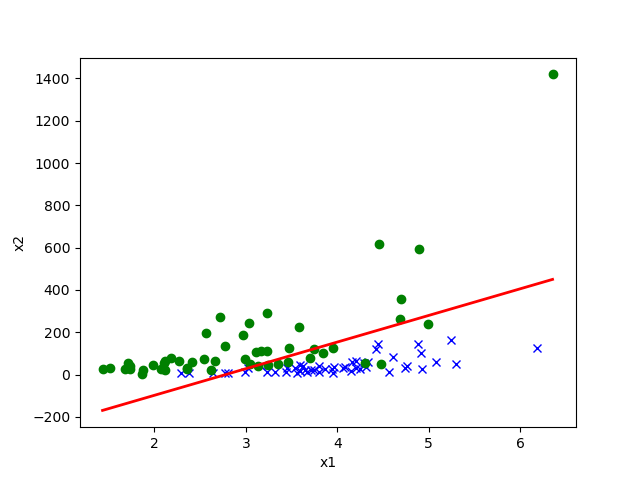
\includegraphics[width=\linewidth]{p01b_pred_1_txt.png}
        \subcaption{Logistic Regression for Dataset 1}
    \end{subfigure}
    \begin{subfigure}[b]{0.5\linewidth}
        \centering
        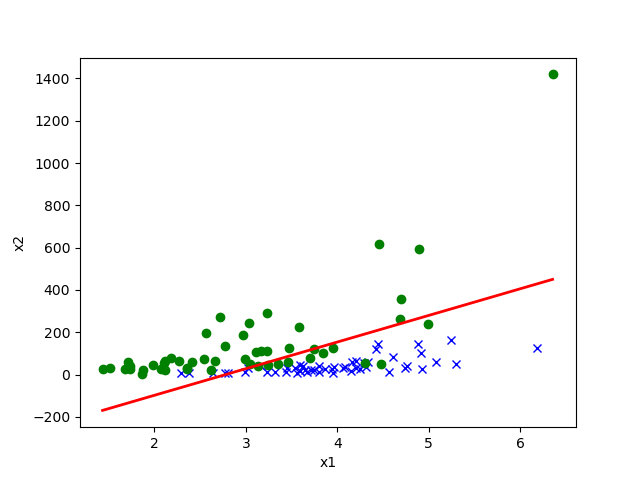
\includegraphics[width=\linewidth]{p01e_pred_1_txt.png}
        \subcaption{GDA for Dataset 1}
    \end{subfigure}

\end{figure}

\end{answer}
} \fi

	\clearpage
\item \subquestionpoints{5}
Repeat the steps in part (f) for Dataset 2. On which dataset does GDA seem to
perform worse than logistic regression? Why might this be the case?

\ifnum\solutions=1{
  \begin{answer}
\begin{figure}[htbp]
    \begin{subfigure}[b]{0.5\linewidth}
        \centering
        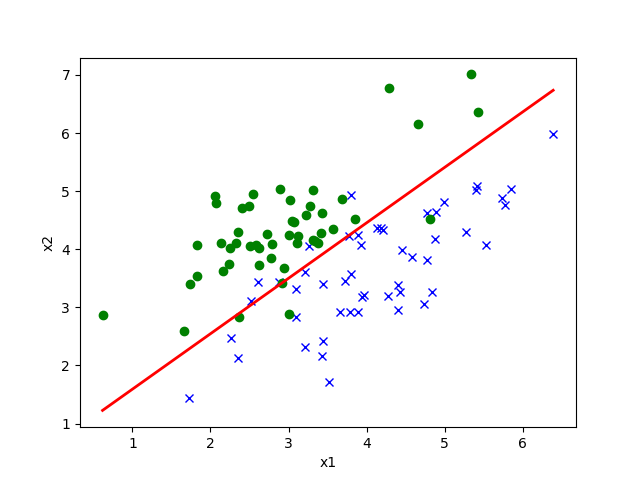
\includegraphics[width=\linewidth]{output/p01b_pred_2.txt.png}
        \subcaption{Logistic Regression for Dataset 2}
    \end{subfigure}
    \begin{subfigure}[b]{0.5\linewidth}
        \centering
        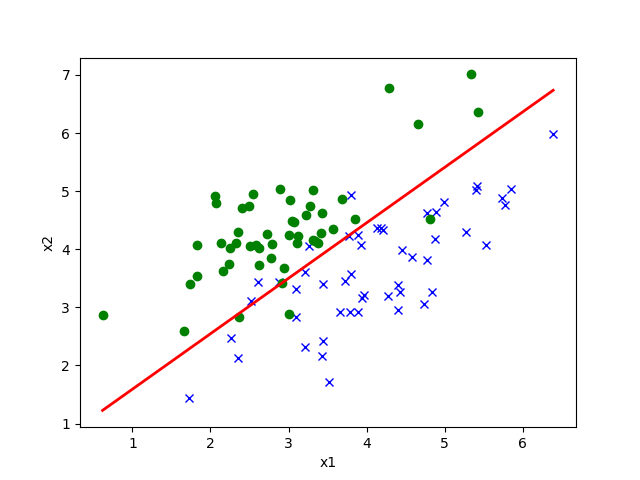
\includegraphics[width=\linewidth]{output/p01e_pred_2.txt.png}
        \subcaption{GDA for Dataset 2}
    \end{subfigure}

\end{figure}
\end{answer}

}\fi

	\clearpage
\item \points{3 extra credit} For the dataset where GDA performed worse in
parts (f) and (g), can you find a transformation of the $x^{(i)}$'s such
that GDA performs significantly better? What is this transformation?

\ifnum\solutions=1{
  \begin{answer}
\end{answer}

}\fi

\end{enumerate}


\clearpage
\item \points{40} {\bf Linear Classifiers (logistic regression and GDA)}

In this problem, we cover two probabilistic linear classifiers we have
covered in class so far. First, a discriminative linear classifier: logistic
regression. Second, a generative linear classifier: Gaussian discriminant
analysis (GDA). Both the algorithms find a linear decision boundary that
separates the data into two classes, but make different assumptions. Our goal
in this problem is to get a deeper understanding of the similarities and
differences (and, strengths and weaknesses) of these two algorithms.

For this problem, we will consider two datasets, provided in the following
files:
\begin{enumerate}[label=\roman*.]
	\item \url{data/ds1_{train,valid}.csv}
	\item \url{data/ds2_{train,valid}.csv}
\end{enumerate}
Each file contains $m$ examples, one example $(x^{(i)}, y^{(i)})$ per row.
In particular, the $i$-th row contains columns $x^{(i)}_0\in\Re$,
$x^{(i)}_1\in\Re$, and $y^{(i)}\in\{0, 1\}$. In the subproblems that follow, we
will investigate using logistic regression and Gaussian discriminant analysis
(GDA) to perform binary classification on these two datasets.

\begin{enumerate}
	\item \subquestionpoints{10}
In lecture we saw the average empirical loss for logistic regression:
\begin{equation*}
	J(\theta)
	= -\frac{1}{m} \sum_{i=1}^m y^{(i)}\log(h_{\theta}(x^{(i)}))
		+  (1 - y^{(i)})\log(1 - h_{\theta}(x^{(i)})),
\end{equation*}
where $y^{(i)} \in \{0, 1\}$, $h_\theta(x) = g(\theta^T x)$ and
$g(z) = 1 / (1 + e^{-z})$.

Find the Hessian $H$ of this function, and show that for any vector $z$, it
holds true that
%
\begin{equation*}
    z^T H z \ge 0.
\end{equation*}
%
{\bf Hint:} You may want to start by showing that
$\sum_i\sum_j z_i x_i x_j z_j = (x^Tz)^2 \geq 0$. Recall also that
$g'(z) = g(z)(1-g(z))$.

{\bf Remark:} This is one of the standard ways of showing that the matrix $H$
is positive semi-definite, written ``$H \succeq 0$.''  This implies that $J$ is
convex, and has no local minima other than the global one. If you have some
other way of showing $H \succeq 0$, you're also welcome to use your method
instead of the one above.

\ifnum\solutions=1 {
  \begin{answer}
Throughout the problem set $(a,b)$ denoted the inner(dot) product of the vectors $a,b.$
It is easy to see that for the logistic function $g(z)$, we have $g'(z)= g(z)(1- g(z)).$ We use this to calculate the partial derivative of the loss functions. 
$$\frac{\partial h_{\theta}(x)}{\partial \theta_i} = \frac{\partial g(\theta^Tx)}{\partial \theta_i} = g(\theta^Tx) (1 - g(\theta^Tx))
\frac{\partial}{\partial\theta_i}(\theta^Tx) = h_{\theta}(x) (1 - h_{\theta}(x)) x_i$$
Hence,

$$\frac{\partial log(h_{\theta}(x))}{\partial \theta_i} = \frac{h'_{\theta}(x)}{h_{\theta}(x)} = (1 - h_{\theta}(x))x_i.$$
Similarly,

$$\frac{\partial (1 - log(1 - h_{\theta}(x)))}{\partial \theta_i} = - \frac{h'_{\theta}(x)}{1 - h_{\theta}(x)} = -h_{\theta}(x)x_i.$$

Using the above computations and some simplification we obtain the partial derivative of the loss function wrt $i-$th component.
$$\frac{\partial J(\theta)}{\partial \theta_i} = - \frac{1}{m}\sum_{k = 1}^{m }x_i^{(k)}( y^{(k)} - h_{\theta}(x^{(k)})). \eqno(1)$$

Note that the above sum can conveniently be expressed in the form of inner product and we will use such form in the coding part using numpy's dot operation.

The formula (1)  allow us to easily find the entries of the Hessian.

$$\frac{\partial^2 J(\theta)}{\partial \theta_i \partial\theta_j} = 
\frac{1}{m}\sum_{k = 0}^{m - 1}g'(\theta^Tx^{(k)}))x_i^{(k)}x_j^{(k)}. \eqno(2)$$
Thus, the $(i,j)-$ th entry  of the Hessian matrix is given by the right hand side of (2).
Now we show that the Hessian is positive semi-definite. Below $(a,b)$ denotes the inner product of $a$ and $b.$
$$z^THz = (Hz,z)=  \sum_{i,j}\sum_{k = 1}^{m}g'(\theta^Tx^{(k)})x_i^{(k)}x_j^{(k)}z_iz_j=  \sum_{k = 1}^m\sum_{i,j}g'(\theta^Tx^{(k)})x_i^{(k)}x_j^{(k)}z_iz_j$$
$$= \sum_{k = 1}^m g'(\theta^Tx^{(k)}) (x^Tz)^2 \ge 0.$$
as the logistic function is non -decreasing so its derivative is non-negative (or $g' = g(1-g)\ge 0$).

\end{answer}

  
} \fi

	\clearpage
\item \subquestionpoints{5} \textbf{Coding problem.}
Follow the instructions in \texttt{src/p01b\_logreg.py} to train a
logistic regression classifier using Newton's Method.
Starting with $\theta = \vec{0}$, run Newton's Method until the updates to
$\theta$ are small: Specifically,  train until the first iteration $k$ such
that $\|\theta_{k} - \theta_{k-1}\|_1 < \epsilon$, where
$\epsilon = 1\times 10^{-5}$. Make sure to write your model's predictions to
the file specified in the code.

\ifnum\solutions=1 {
  \begin{answer}
Done!
\end{answer}

} \fi

	\clearpage
\item \subquestionpoints{5}
Recall that in GDA we model the joint distribution of $(x, y)$ by the following
equations:
%
\begin{eqnarray*}
	p(y) &=& \begin{cases}
	\phi & \mbox{if~} y = 1 \\
	1 - \phi & \mbox{if~} y = 0 \end{cases} \\
	p(x | y=0) &=& \frac{1}{(2\pi)^{n/2} |\Sigma|^{1/2}}
		\exp\left(-\frac{1}{2}(x-\mu_{0})^T \Sigma^{-1} (x-\mu_{0})\right) \\
	p(x | y=1) &=& \frac{1}{(2\pi)^{n/2} |\Sigma|^{1/2}}
		\exp\left(-\frac{1}{2}(x-\mu_1)^T \Sigma^{-1} (x-\mu_1) \right),
\end{eqnarray*}
%
where $\phi$, $\mu_0$, $\mu_1$, and $\Sigma$ are the parameters of our model.

Suppose we have already fit $\phi$, $\mu_0$, $\mu_1$, and $\Sigma$, and now
want to predict $y$ given a new point $x$. To show that GDA results in a
classifier that has a linear decision boundary, show the posterior distribution
can be written as
%
\begin{equation*}
	p(y = 1\mid x; \phi, \mu_0, \mu_1, \Sigma)
	= \frac{1}{1 + \exp(-(\theta^T x + \theta_0))},
\end{equation*}
%
where $\theta\in\Re^n$ and $\theta_{0}\in\Re$ are appropriate functions of
$\phi$, $\Sigma$, $\mu_0$, and $\mu_1$.

\ifnum\solutions=1{
  \begin{answer}
Apply Bayes
$$p(y = 1| x) = \frac{p(x| y=1)p(y = 1)}{p(x| y=1)p(y = 1) + p(x| y=0)p(y = 0)} = \frac{1}{1 + \frac{p(x| y=0)p(y = 0)}{p(x| y=1)p(y = 1)}}.$$
Note that $\frac{p(y = 0)}{p(y = 1)} = exp(ln(\frac{1-\phi}{\phi})$
For simplicity  denote A = $\Sigma^{-1}.$
Note that
$$\frac{p(x| y=0)}{p(x| y=1)} = exp(-\frac{1}{2}(A(x- \mu_0), x - \mu_0) - (A(x- \mu_1), x - \mu_1))) $$$$= exp(-\frac 12((Ax,x) - 2(Ax, \mu_0) + (\mu_0, \mu_0) - (Ax,x) + 2(Ax, \mu_1) + (\mu_1, \mu_1)))$$
$$= exp(-( -(Ax, \mu_0) + \frac 12(A\mu_0, \mu_0) + (Ax, \mu_1) - \frac12(A\mu_1, \mu_1))) = exp(-(\mu_1 - \mu_0)^TAx + \frac{1}{2}((A\mu_0,\mu_0) - (A\mu_1,\mu_1)).$$
From this we find $\theta^T = (\mu_1 - \mu_0)^TA$ hence 
$$\theta = (\Sigma^{-1})^T(\mu_1 - \mu_0)$$
and
$$\theta_0 = \frac{1}{2}((\Sigma^{-1}\mu_0,\mu_0) - (\Sigma^{-1}\mu_1,\mu_1)) - ln(\frac{1-\phi}{\phi}).$$

\end{answer}

}\fi

	\clearpage
\item \subquestionpoints{7} For this part of the problem only, you may
  assume $n$ (the dimension of $x$) is 1, so that $\Sigma = [\sigma^2]$ is
  just a real number, and likewise the determinant of $\Sigma$ is given by
  $|\Sigma| = \sigma^2$.  Given the dataset, we claim that the maximum
  likelihood estimates of the parameters are given by
  \begin{eqnarray*}
    \phi &=& \frac{1}{m} \sum_{i=1}^m 1\{y^{(i)} = 1\} \\
\mu_{0} &=& \frac{\sum_{i=1}^m 1\{y^{(i)} = {0}\} x^{(i)}}{\sum_{i=1}^m
1\{y^{(i)} = {0}\}} \\
\mu_1 &=& \frac{\sum_{i=1}^m 1\{y^{(i)} = 1\} x^{(i)}}{\sum_{i=1}^m 1\{y^{(i)}
= 1\}} \\
\Sigma &=& \frac{1}{m} \sum_{i=1}^m (x^{(i)} - \mu_{y^{(i)}}) (x^{(i)} -
\mu_{y^{(i)}})^T
  \end{eqnarray*}
  The log-likelihood of the data is
  \begin{eqnarray*}
\ell(\phi, \mu_{0}, \mu_1, \Sigma) &=& \log \prod_{i=1}^m p(x^{(i)} , y^{(i)};
\phi, \mu_{0}, \mu_1, \Sigma) \\
&=& \log \prod_{i=1}^m p(x^{(i)} | y^{(i)}; \mu_{0}, \mu_1, \Sigma) p(y^{(i)};
\phi).
  \end{eqnarray*}
By maximizing $\ell$ with respect to the four parameters,
prove that the maximum likelihood estimates of $\phi$, $\mu_{0}, \mu_1$, and
$\Sigma$ are indeed as given in the formulas above.  (You may assume that there
is at least one positive and one negative example, so that the denominators in
the definitions of $\mu_{0}$ and $\mu_1$ above are non-zero.)

\ifnum\solutions=1 {
  \begin{answer}
The product and the sums run from  1 to m, so for simplicity I drop the limits. Note that
$$l = \log\prod p(y^{(i)}| x^{(i)})p(y{(i)}) = \sum\log p(y^{(i)}| x^{(i)})p(y{(i)}) = $$$$
 -m\log(\sigma) + c_0 - \sum\big( y^{(i)}\frac{(x^{(i)} - \mu_0)^2}{2\sigma^2} + (1- y^{(i)})\frac{(x^{(i)} - \mu_1)^2}{2\sigma^2}\big) + \sum(y^{(i)}\phi + (1-y^{(i)})(1-\phi)).$$
 
 Now we calculate the partial derivatives.
 
 $$\frac{\partial}{\partial\phi} = \sum(\frac{y^{(i)}}{\phi} + \frac{1- y^{(i)}}{1-\phi}) = 0.$$
 The numerator after the sum is then $\sum y^{(i)} - m\phi$ and so
 $$\phi= \frac{\sum y^{(i)}}{m}.$$
 Not that the formula is exactly as the formula given in the problem because if $y^{(i)} = 0$ the $i-$th term of the sum is $0.$ Hence this formula can be represented with the characteristic function. I will not be re-writing this as well as the problems below as I do not know how useful it may be in the coding part.
 Further derivatives (enough to show $\mu_0$):
 $$\frac{\partial l}{\partial\mu_0} =\sum\frac{y^{(i)}(x^{(i)} - \mu_0 )}{\sigma^2} = \frac{\sum x^{(i)}y^{(i)} - \mu_0\sum y^{(i)}}{\sigma^2}.$$
 Hence we obtain
 $$\mu_0 = \frac{\sum x^{(i)}y^{(i)}}{\sum y^{(i)}}.$$
 Finally, 
 $$\frac{\partial l}{\partial \sigma} = \frac{m}{\sigma} - \frac{1}{\sigma^3}(\sum\big( y^{(i)}\frac{(x^{(i)} - \mu_0)^2}{2\sigma^2} + (1- y^{(i)})\frac{(x^{(i)} - \mu_1)^2}{2\sigma^2}\big)).$$
 By solving this equation for $\sigma$ we obtain the desired result.
 
 
 
\end{answer}

} \fi

	\clearpage
\item \subquestionpoints{3} \textbf{Coding problem.}
In \texttt{src/p01e\_gda.py}, fill in the code to
calculate $\phi$, $\mu_{0}$, $\mu_{1}$, and $\Sigma$, use these parameters
to derive $\theta$, and use the resulting GDA model to make predictions on the
validation set.

\ifnum\solutions=1 {
  \begin{answer}
\end{answer}

} \fi

	\clearpage
\item \subquestionpoints{5}
For Dataset 1, create a plot of the validation set with $x_1$ on the horizontal
axis, and $x_2$ on the vertical axis. To visualize the two classes, use a
different symbol for examples $x^{(i)}$ with $y^{(i)} = 0$ than for those with
$y^{(i)} = 1$. On the same figure, plot the decision boundary found by logistic
regression in part (b). Make an identical plot with the decision boundary found
by GDA in part (e).

\ifnum\solutions=1 {
  
\begin{answer}
\begin{figure}[htbp]
    \begin{subfigure}[b]{0.5\linewidth}
        \centering
        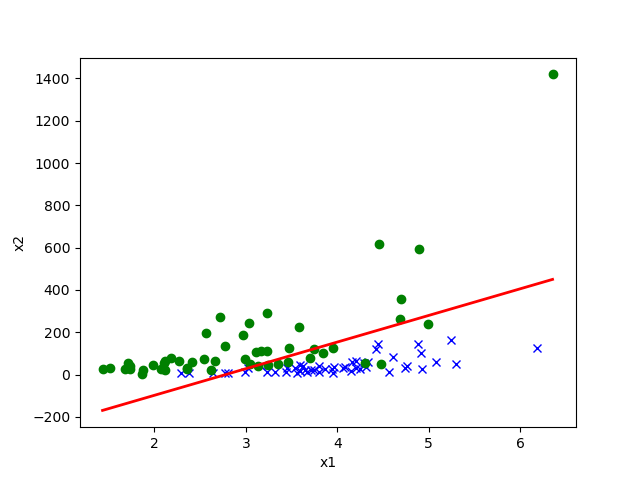
\includegraphics[width=\linewidth]{p01b_pred_1_txt.png}
        \subcaption{Logistic Regression for Dataset 1}
    \end{subfigure}
    \begin{subfigure}[b]{0.5\linewidth}
        \centering
        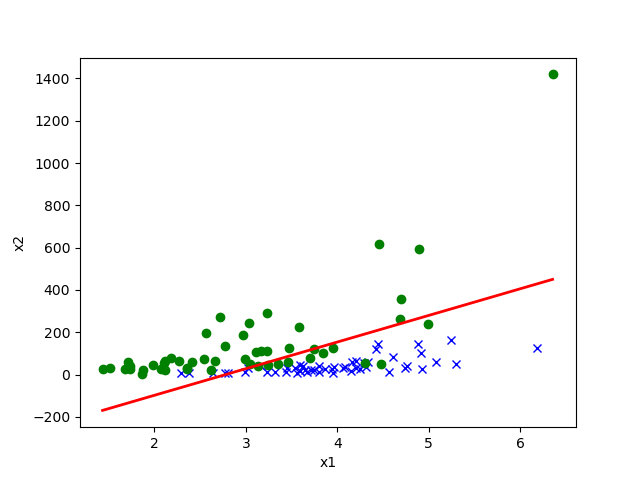
\includegraphics[width=\linewidth]{p01e_pred_1_txt.png}
        \subcaption{GDA for Dataset 1}
    \end{subfigure}

\end{figure}

\end{answer}
} \fi

	\clearpage
\item \subquestionpoints{5}
Repeat the steps in part (f) for Dataset 2. On which dataset does GDA seem to
perform worse than logistic regression? Why might this be the case?

\ifnum\solutions=1{
  \begin{answer}
\begin{figure}[htbp]
    \begin{subfigure}[b]{0.5\linewidth}
        \centering
        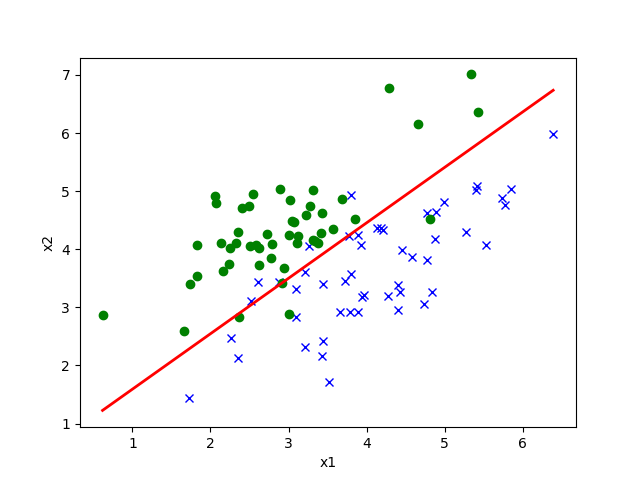
\includegraphics[width=\linewidth]{output/p01b_pred_2.txt.png}
        \subcaption{Logistic Regression for Dataset 2}
    \end{subfigure}
    \begin{subfigure}[b]{0.5\linewidth}
        \centering
        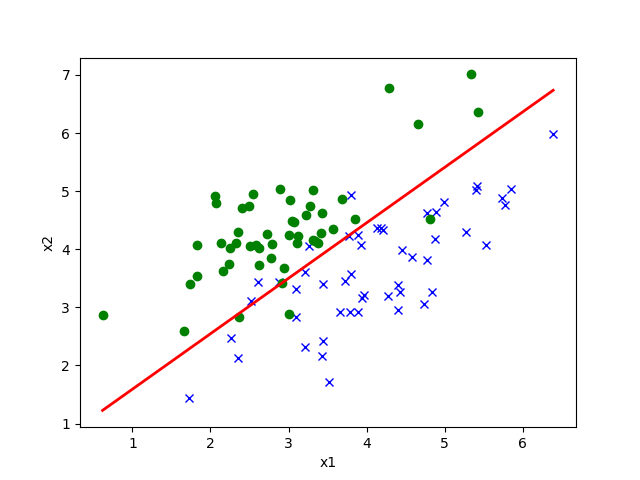
\includegraphics[width=\linewidth]{output/p01e_pred_2.txt.png}
        \subcaption{GDA for Dataset 2}
    \end{subfigure}

\end{figure}
\end{answer}

}\fi

	\clearpage
\item \points{3 extra credit} For the dataset where GDA performed worse in
parts (f) and (g), can you find a transformation of the $x^{(i)}$'s such
that GDA performs significantly better? What is this transformation?

\ifnum\solutions=1{
  \begin{answer}
\end{answer}

}\fi

\end{enumerate}


\clearpage
\item \points{40} {\bf Linear Classifiers (logistic regression and GDA)}

In this problem, we cover two probabilistic linear classifiers we have
covered in class so far. First, a discriminative linear classifier: logistic
regression. Second, a generative linear classifier: Gaussian discriminant
analysis (GDA). Both the algorithms find a linear decision boundary that
separates the data into two classes, but make different assumptions. Our goal
in this problem is to get a deeper understanding of the similarities and
differences (and, strengths and weaknesses) of these two algorithms.

For this problem, we will consider two datasets, provided in the following
files:
\begin{enumerate}[label=\roman*.]
	\item \url{data/ds1_{train,valid}.csv}
	\item \url{data/ds2_{train,valid}.csv}
\end{enumerate}
Each file contains $m$ examples, one example $(x^{(i)}, y^{(i)})$ per row.
In particular, the $i$-th row contains columns $x^{(i)}_0\in\Re$,
$x^{(i)}_1\in\Re$, and $y^{(i)}\in\{0, 1\}$. In the subproblems that follow, we
will investigate using logistic regression and Gaussian discriminant analysis
(GDA) to perform binary classification on these two datasets.

\begin{enumerate}
	\item \subquestionpoints{10}
In lecture we saw the average empirical loss for logistic regression:
\begin{equation*}
	J(\theta)
	= -\frac{1}{m} \sum_{i=1}^m y^{(i)}\log(h_{\theta}(x^{(i)}))
		+  (1 - y^{(i)})\log(1 - h_{\theta}(x^{(i)})),
\end{equation*}
where $y^{(i)} \in \{0, 1\}$, $h_\theta(x) = g(\theta^T x)$ and
$g(z) = 1 / (1 + e^{-z})$.

Find the Hessian $H$ of this function, and show that for any vector $z$, it
holds true that
%
\begin{equation*}
    z^T H z \ge 0.
\end{equation*}
%
{\bf Hint:} You may want to start by showing that
$\sum_i\sum_j z_i x_i x_j z_j = (x^Tz)^2 \geq 0$. Recall also that
$g'(z) = g(z)(1-g(z))$.

{\bf Remark:} This is one of the standard ways of showing that the matrix $H$
is positive semi-definite, written ``$H \succeq 0$.''  This implies that $J$ is
convex, and has no local minima other than the global one. If you have some
other way of showing $H \succeq 0$, you're also welcome to use your method
instead of the one above.

\ifnum\solutions=1 {
  \begin{answer}
Throughout the problem set $(a,b)$ denoted the inner(dot) product of the vectors $a,b.$
It is easy to see that for the logistic function $g(z)$, we have $g'(z)= g(z)(1- g(z)).$ We use this to calculate the partial derivative of the loss functions. 
$$\frac{\partial h_{\theta}(x)}{\partial \theta_i} = \frac{\partial g(\theta^Tx)}{\partial \theta_i} = g(\theta^Tx) (1 - g(\theta^Tx))
\frac{\partial}{\partial\theta_i}(\theta^Tx) = h_{\theta}(x) (1 - h_{\theta}(x)) x_i$$
Hence,

$$\frac{\partial log(h_{\theta}(x))}{\partial \theta_i} = \frac{h'_{\theta}(x)}{h_{\theta}(x)} = (1 - h_{\theta}(x))x_i.$$
Similarly,

$$\frac{\partial (1 - log(1 - h_{\theta}(x)))}{\partial \theta_i} = - \frac{h'_{\theta}(x)}{1 - h_{\theta}(x)} = -h_{\theta}(x)x_i.$$

Using the above computations and some simplification we obtain the partial derivative of the loss function wrt $i-$th component.
$$\frac{\partial J(\theta)}{\partial \theta_i} = - \frac{1}{m}\sum_{k = 1}^{m }x_i^{(k)}( y^{(k)} - h_{\theta}(x^{(k)})). \eqno(1)$$

Note that the above sum can conveniently be expressed in the form of inner product and we will use such form in the coding part using numpy's dot operation.

The formula (1)  allow us to easily find the entries of the Hessian.

$$\frac{\partial^2 J(\theta)}{\partial \theta_i \partial\theta_j} = 
\frac{1}{m}\sum_{k = 0}^{m - 1}g'(\theta^Tx^{(k)}))x_i^{(k)}x_j^{(k)}. \eqno(2)$$
Thus, the $(i,j)-$ th entry  of the Hessian matrix is given by the right hand side of (2).
Now we show that the Hessian is positive semi-definite. Below $(a,b)$ denotes the inner product of $a$ and $b.$
$$z^THz = (Hz,z)=  \sum_{i,j}\sum_{k = 1}^{m}g'(\theta^Tx^{(k)})x_i^{(k)}x_j^{(k)}z_iz_j=  \sum_{k = 1}^m\sum_{i,j}g'(\theta^Tx^{(k)})x_i^{(k)}x_j^{(k)}z_iz_j$$
$$= \sum_{k = 1}^m g'(\theta^Tx^{(k)}) (x^Tz)^2 \ge 0.$$
as the logistic function is non -decreasing so its derivative is non-negative (or $g' = g(1-g)\ge 0$).

\end{answer}

  
} \fi

	\clearpage
\item \subquestionpoints{5} \textbf{Coding problem.}
Follow the instructions in \texttt{src/p01b\_logreg.py} to train a
logistic regression classifier using Newton's Method.
Starting with $\theta = \vec{0}$, run Newton's Method until the updates to
$\theta$ are small: Specifically,  train until the first iteration $k$ such
that $\|\theta_{k} - \theta_{k-1}\|_1 < \epsilon$, where
$\epsilon = 1\times 10^{-5}$. Make sure to write your model's predictions to
the file specified in the code.

\ifnum\solutions=1 {
  \begin{answer}
Done!
\end{answer}

} \fi

	\clearpage
\item \subquestionpoints{5}
Recall that in GDA we model the joint distribution of $(x, y)$ by the following
equations:
%
\begin{eqnarray*}
	p(y) &=& \begin{cases}
	\phi & \mbox{if~} y = 1 \\
	1 - \phi & \mbox{if~} y = 0 \end{cases} \\
	p(x | y=0) &=& \frac{1}{(2\pi)^{n/2} |\Sigma|^{1/2}}
		\exp\left(-\frac{1}{2}(x-\mu_{0})^T \Sigma^{-1} (x-\mu_{0})\right) \\
	p(x | y=1) &=& \frac{1}{(2\pi)^{n/2} |\Sigma|^{1/2}}
		\exp\left(-\frac{1}{2}(x-\mu_1)^T \Sigma^{-1} (x-\mu_1) \right),
\end{eqnarray*}
%
where $\phi$, $\mu_0$, $\mu_1$, and $\Sigma$ are the parameters of our model.

Suppose we have already fit $\phi$, $\mu_0$, $\mu_1$, and $\Sigma$, and now
want to predict $y$ given a new point $x$. To show that GDA results in a
classifier that has a linear decision boundary, show the posterior distribution
can be written as
%
\begin{equation*}
	p(y = 1\mid x; \phi, \mu_0, \mu_1, \Sigma)
	= \frac{1}{1 + \exp(-(\theta^T x + \theta_0))},
\end{equation*}
%
where $\theta\in\Re^n$ and $\theta_{0}\in\Re$ are appropriate functions of
$\phi$, $\Sigma$, $\mu_0$, and $\mu_1$.

\ifnum\solutions=1{
  \begin{answer}
Apply Bayes
$$p(y = 1| x) = \frac{p(x| y=1)p(y = 1)}{p(x| y=1)p(y = 1) + p(x| y=0)p(y = 0)} = \frac{1}{1 + \frac{p(x| y=0)p(y = 0)}{p(x| y=1)p(y = 1)}}.$$
Note that $\frac{p(y = 0)}{p(y = 1)} = exp(ln(\frac{1-\phi}{\phi})$
For simplicity  denote A = $\Sigma^{-1}.$
Note that
$$\frac{p(x| y=0)}{p(x| y=1)} = exp(-\frac{1}{2}(A(x- \mu_0), x - \mu_0) - (A(x- \mu_1), x - \mu_1))) $$$$= exp(-\frac 12((Ax,x) - 2(Ax, \mu_0) + (\mu_0, \mu_0) - (Ax,x) + 2(Ax, \mu_1) + (\mu_1, \mu_1)))$$
$$= exp(-( -(Ax, \mu_0) + \frac 12(A\mu_0, \mu_0) + (Ax, \mu_1) - \frac12(A\mu_1, \mu_1))) = exp(-(\mu_1 - \mu_0)^TAx + \frac{1}{2}((A\mu_0,\mu_0) - (A\mu_1,\mu_1)).$$
From this we find $\theta^T = (\mu_1 - \mu_0)^TA$ hence 
$$\theta = (\Sigma^{-1})^T(\mu_1 - \mu_0)$$
and
$$\theta_0 = \frac{1}{2}((\Sigma^{-1}\mu_0,\mu_0) - (\Sigma^{-1}\mu_1,\mu_1)) - ln(\frac{1-\phi}{\phi}).$$

\end{answer}

}\fi

	\clearpage
\item \subquestionpoints{7} For this part of the problem only, you may
  assume $n$ (the dimension of $x$) is 1, so that $\Sigma = [\sigma^2]$ is
  just a real number, and likewise the determinant of $\Sigma$ is given by
  $|\Sigma| = \sigma^2$.  Given the dataset, we claim that the maximum
  likelihood estimates of the parameters are given by
  \begin{eqnarray*}
    \phi &=& \frac{1}{m} \sum_{i=1}^m 1\{y^{(i)} = 1\} \\
\mu_{0} &=& \frac{\sum_{i=1}^m 1\{y^{(i)} = {0}\} x^{(i)}}{\sum_{i=1}^m
1\{y^{(i)} = {0}\}} \\
\mu_1 &=& \frac{\sum_{i=1}^m 1\{y^{(i)} = 1\} x^{(i)}}{\sum_{i=1}^m 1\{y^{(i)}
= 1\}} \\
\Sigma &=& \frac{1}{m} \sum_{i=1}^m (x^{(i)} - \mu_{y^{(i)}}) (x^{(i)} -
\mu_{y^{(i)}})^T
  \end{eqnarray*}
  The log-likelihood of the data is
  \begin{eqnarray*}
\ell(\phi, \mu_{0}, \mu_1, \Sigma) &=& \log \prod_{i=1}^m p(x^{(i)} , y^{(i)};
\phi, \mu_{0}, \mu_1, \Sigma) \\
&=& \log \prod_{i=1}^m p(x^{(i)} | y^{(i)}; \mu_{0}, \mu_1, \Sigma) p(y^{(i)};
\phi).
  \end{eqnarray*}
By maximizing $\ell$ with respect to the four parameters,
prove that the maximum likelihood estimates of $\phi$, $\mu_{0}, \mu_1$, and
$\Sigma$ are indeed as given in the formulas above.  (You may assume that there
is at least one positive and one negative example, so that the denominators in
the definitions of $\mu_{0}$ and $\mu_1$ above are non-zero.)

\ifnum\solutions=1 {
  \begin{answer}
The product and the sums run from  1 to m, so for simplicity I drop the limits. Note that
$$l = \log\prod p(y^{(i)}| x^{(i)})p(y{(i)}) = \sum\log p(y^{(i)}| x^{(i)})p(y{(i)}) = $$$$
 -m\log(\sigma) + c_0 - \sum\big( y^{(i)}\frac{(x^{(i)} - \mu_0)^2}{2\sigma^2} + (1- y^{(i)})\frac{(x^{(i)} - \mu_1)^2}{2\sigma^2}\big) + \sum(y^{(i)}\phi + (1-y^{(i)})(1-\phi)).$$
 
 Now we calculate the partial derivatives.
 
 $$\frac{\partial}{\partial\phi} = \sum(\frac{y^{(i)}}{\phi} + \frac{1- y^{(i)}}{1-\phi}) = 0.$$
 The numerator after the sum is then $\sum y^{(i)} - m\phi$ and so
 $$\phi= \frac{\sum y^{(i)}}{m}.$$
 Not that the formula is exactly as the formula given in the problem because if $y^{(i)} = 0$ the $i-$th term of the sum is $0.$ Hence this formula can be represented with the characteristic function. I will not be re-writing this as well as the problems below as I do not know how useful it may be in the coding part.
 Further derivatives (enough to show $\mu_0$):
 $$\frac{\partial l}{\partial\mu_0} =\sum\frac{y^{(i)}(x^{(i)} - \mu_0 )}{\sigma^2} = \frac{\sum x^{(i)}y^{(i)} - \mu_0\sum y^{(i)}}{\sigma^2}.$$
 Hence we obtain
 $$\mu_0 = \frac{\sum x^{(i)}y^{(i)}}{\sum y^{(i)}}.$$
 Finally, 
 $$\frac{\partial l}{\partial \sigma} = \frac{m}{\sigma} - \frac{1}{\sigma^3}(\sum\big( y^{(i)}\frac{(x^{(i)} - \mu_0)^2}{2\sigma^2} + (1- y^{(i)})\frac{(x^{(i)} - \mu_1)^2}{2\sigma^2}\big)).$$
 By solving this equation for $\sigma$ we obtain the desired result.
 
 
 
\end{answer}

} \fi

	\clearpage
\item \subquestionpoints{3} \textbf{Coding problem.}
In \texttt{src/p01e\_gda.py}, fill in the code to
calculate $\phi$, $\mu_{0}$, $\mu_{1}$, and $\Sigma$, use these parameters
to derive $\theta$, and use the resulting GDA model to make predictions on the
validation set.

\ifnum\solutions=1 {
  \begin{answer}
\end{answer}

} \fi

	\clearpage
\item \subquestionpoints{5}
For Dataset 1, create a plot of the validation set with $x_1$ on the horizontal
axis, and $x_2$ on the vertical axis. To visualize the two classes, use a
different symbol for examples $x^{(i)}$ with $y^{(i)} = 0$ than for those with
$y^{(i)} = 1$. On the same figure, plot the decision boundary found by logistic
regression in part (b). Make an identical plot with the decision boundary found
by GDA in part (e).

\ifnum\solutions=1 {
  
\begin{answer}
\begin{figure}[htbp]
    \begin{subfigure}[b]{0.5\linewidth}
        \centering
        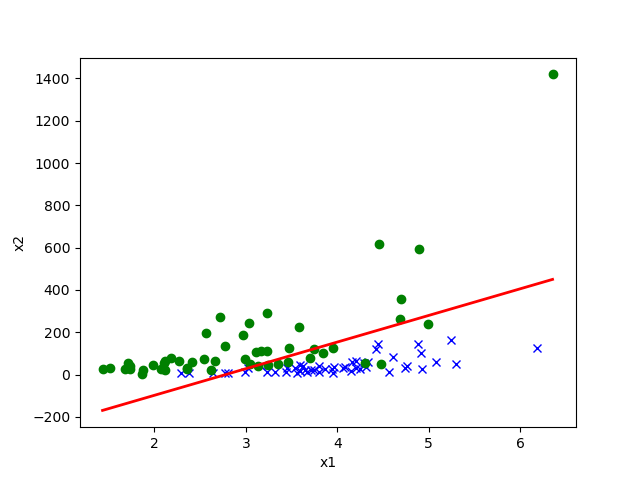
\includegraphics[width=\linewidth]{p01b_pred_1_txt.png}
        \subcaption{Logistic Regression for Dataset 1}
    \end{subfigure}
    \begin{subfigure}[b]{0.5\linewidth}
        \centering
        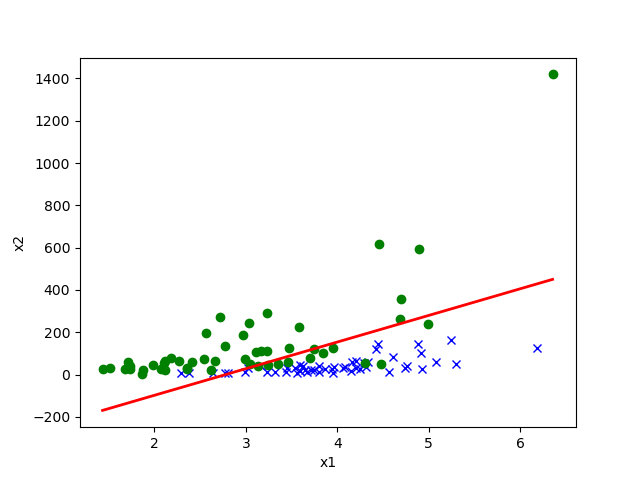
\includegraphics[width=\linewidth]{p01e_pred_1_txt.png}
        \subcaption{GDA for Dataset 1}
    \end{subfigure}

\end{figure}

\end{answer}
} \fi

	\clearpage
\item \subquestionpoints{5}
Repeat the steps in part (f) for Dataset 2. On which dataset does GDA seem to
perform worse than logistic regression? Why might this be the case?

\ifnum\solutions=1{
  \begin{answer}
\begin{figure}[htbp]
    \begin{subfigure}[b]{0.5\linewidth}
        \centering
        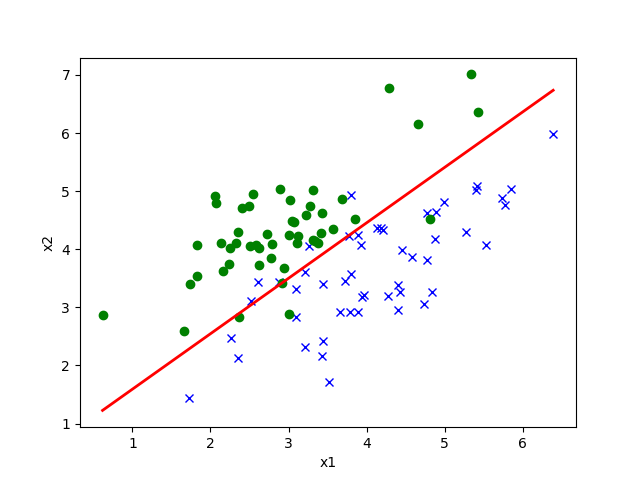
\includegraphics[width=\linewidth]{output/p01b_pred_2.txt.png}
        \subcaption{Logistic Regression for Dataset 2}
    \end{subfigure}
    \begin{subfigure}[b]{0.5\linewidth}
        \centering
        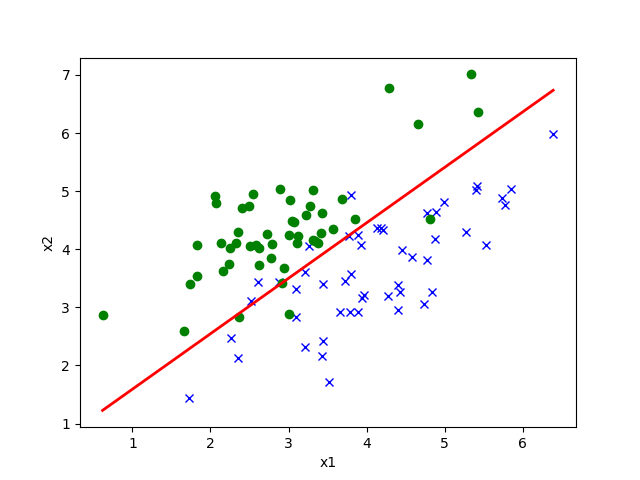
\includegraphics[width=\linewidth]{output/p01e_pred_2.txt.png}
        \subcaption{GDA for Dataset 2}
    \end{subfigure}

\end{figure}
\end{answer}

}\fi

	\clearpage
\item \points{3 extra credit} For the dataset where GDA performed worse in
parts (f) and (g), can you find a transformation of the $x^{(i)}$'s such
that GDA performs significantly better? What is this transformation?

\ifnum\solutions=1{
  \begin{answer}
\end{answer}

}\fi

\end{enumerate}


\clearpage
\item \points{40} {\bf Linear Classifiers (logistic regression and GDA)}

In this problem, we cover two probabilistic linear classifiers we have
covered in class so far. First, a discriminative linear classifier: logistic
regression. Second, a generative linear classifier: Gaussian discriminant
analysis (GDA). Both the algorithms find a linear decision boundary that
separates the data into two classes, but make different assumptions. Our goal
in this problem is to get a deeper understanding of the similarities and
differences (and, strengths and weaknesses) of these two algorithms.

For this problem, we will consider two datasets, provided in the following
files:
\begin{enumerate}[label=\roman*.]
	\item \url{data/ds1_{train,valid}.csv}
	\item \url{data/ds2_{train,valid}.csv}
\end{enumerate}
Each file contains $m$ examples, one example $(x^{(i)}, y^{(i)})$ per row.
In particular, the $i$-th row contains columns $x^{(i)}_0\in\Re$,
$x^{(i)}_1\in\Re$, and $y^{(i)}\in\{0, 1\}$. In the subproblems that follow, we
will investigate using logistic regression and Gaussian discriminant analysis
(GDA) to perform binary classification on these two datasets.

\begin{enumerate}
	\item \subquestionpoints{10}
In lecture we saw the average empirical loss for logistic regression:
\begin{equation*}
	J(\theta)
	= -\frac{1}{m} \sum_{i=1}^m y^{(i)}\log(h_{\theta}(x^{(i)}))
		+  (1 - y^{(i)})\log(1 - h_{\theta}(x^{(i)})),
\end{equation*}
where $y^{(i)} \in \{0, 1\}$, $h_\theta(x) = g(\theta^T x)$ and
$g(z) = 1 / (1 + e^{-z})$.

Find the Hessian $H$ of this function, and show that for any vector $z$, it
holds true that
%
\begin{equation*}
    z^T H z \ge 0.
\end{equation*}
%
{\bf Hint:} You may want to start by showing that
$\sum_i\sum_j z_i x_i x_j z_j = (x^Tz)^2 \geq 0$. Recall also that
$g'(z) = g(z)(1-g(z))$.

{\bf Remark:} This is one of the standard ways of showing that the matrix $H$
is positive semi-definite, written ``$H \succeq 0$.''  This implies that $J$ is
convex, and has no local minima other than the global one. If you have some
other way of showing $H \succeq 0$, you're also welcome to use your method
instead of the one above.

\ifnum\solutions=1 {
  \begin{answer}
Throughout the problem set $(a,b)$ denoted the inner(dot) product of the vectors $a,b.$
It is easy to see that for the logistic function $g(z)$, we have $g'(z)= g(z)(1- g(z)).$ We use this to calculate the partial derivative of the loss functions. 
$$\frac{\partial h_{\theta}(x)}{\partial \theta_i} = \frac{\partial g(\theta^Tx)}{\partial \theta_i} = g(\theta^Tx) (1 - g(\theta^Tx))
\frac{\partial}{\partial\theta_i}(\theta^Tx) = h_{\theta}(x) (1 - h_{\theta}(x)) x_i$$
Hence,

$$\frac{\partial log(h_{\theta}(x))}{\partial \theta_i} = \frac{h'_{\theta}(x)}{h_{\theta}(x)} = (1 - h_{\theta}(x))x_i.$$
Similarly,

$$\frac{\partial (1 - log(1 - h_{\theta}(x)))}{\partial \theta_i} = - \frac{h'_{\theta}(x)}{1 - h_{\theta}(x)} = -h_{\theta}(x)x_i.$$

Using the above computations and some simplification we obtain the partial derivative of the loss function wrt $i-$th component.
$$\frac{\partial J(\theta)}{\partial \theta_i} = - \frac{1}{m}\sum_{k = 1}^{m }x_i^{(k)}( y^{(k)} - h_{\theta}(x^{(k)})). \eqno(1)$$

Note that the above sum can conveniently be expressed in the form of inner product and we will use such form in the coding part using numpy's dot operation.

The formula (1)  allow us to easily find the entries of the Hessian.

$$\frac{\partial^2 J(\theta)}{\partial \theta_i \partial\theta_j} = 
\frac{1}{m}\sum_{k = 0}^{m - 1}g'(\theta^Tx^{(k)}))x_i^{(k)}x_j^{(k)}. \eqno(2)$$
Thus, the $(i,j)-$ th entry  of the Hessian matrix is given by the right hand side of (2).
Now we show that the Hessian is positive semi-definite. Below $(a,b)$ denotes the inner product of $a$ and $b.$
$$z^THz = (Hz,z)=  \sum_{i,j}\sum_{k = 1}^{m}g'(\theta^Tx^{(k)})x_i^{(k)}x_j^{(k)}z_iz_j=  \sum_{k = 1}^m\sum_{i,j}g'(\theta^Tx^{(k)})x_i^{(k)}x_j^{(k)}z_iz_j$$
$$= \sum_{k = 1}^m g'(\theta^Tx^{(k)}) (x^Tz)^2 \ge 0.$$
as the logistic function is non -decreasing so its derivative is non-negative (or $g' = g(1-g)\ge 0$).

\end{answer}

  
} \fi

	\clearpage
\item \subquestionpoints{5} \textbf{Coding problem.}
Follow the instructions in \texttt{src/p01b\_logreg.py} to train a
logistic regression classifier using Newton's Method.
Starting with $\theta = \vec{0}$, run Newton's Method until the updates to
$\theta$ are small: Specifically,  train until the first iteration $k$ such
that $\|\theta_{k} - \theta_{k-1}\|_1 < \epsilon$, where
$\epsilon = 1\times 10^{-5}$. Make sure to write your model's predictions to
the file specified in the code.

\ifnum\solutions=1 {
  \begin{answer}
Done!
\end{answer}

} \fi

	\clearpage
\item \subquestionpoints{5}
Recall that in GDA we model the joint distribution of $(x, y)$ by the following
equations:
%
\begin{eqnarray*}
	p(y) &=& \begin{cases}
	\phi & \mbox{if~} y = 1 \\
	1 - \phi & \mbox{if~} y = 0 \end{cases} \\
	p(x | y=0) &=& \frac{1}{(2\pi)^{n/2} |\Sigma|^{1/2}}
		\exp\left(-\frac{1}{2}(x-\mu_{0})^T \Sigma^{-1} (x-\mu_{0})\right) \\
	p(x | y=1) &=& \frac{1}{(2\pi)^{n/2} |\Sigma|^{1/2}}
		\exp\left(-\frac{1}{2}(x-\mu_1)^T \Sigma^{-1} (x-\mu_1) \right),
\end{eqnarray*}
%
where $\phi$, $\mu_0$, $\mu_1$, and $\Sigma$ are the parameters of our model.

Suppose we have already fit $\phi$, $\mu_0$, $\mu_1$, and $\Sigma$, and now
want to predict $y$ given a new point $x$. To show that GDA results in a
classifier that has a linear decision boundary, show the posterior distribution
can be written as
%
\begin{equation*}
	p(y = 1\mid x; \phi, \mu_0, \mu_1, \Sigma)
	= \frac{1}{1 + \exp(-(\theta^T x + \theta_0))},
\end{equation*}
%
where $\theta\in\Re^n$ and $\theta_{0}\in\Re$ are appropriate functions of
$\phi$, $\Sigma$, $\mu_0$, and $\mu_1$.

\ifnum\solutions=1{
  \begin{answer}
Apply Bayes
$$p(y = 1| x) = \frac{p(x| y=1)p(y = 1)}{p(x| y=1)p(y = 1) + p(x| y=0)p(y = 0)} = \frac{1}{1 + \frac{p(x| y=0)p(y = 0)}{p(x| y=1)p(y = 1)}}.$$
Note that $\frac{p(y = 0)}{p(y = 1)} = exp(ln(\frac{1-\phi}{\phi})$
For simplicity  denote A = $\Sigma^{-1}.$
Note that
$$\frac{p(x| y=0)}{p(x| y=1)} = exp(-\frac{1}{2}(A(x- \mu_0), x - \mu_0) - (A(x- \mu_1), x - \mu_1))) $$$$= exp(-\frac 12((Ax,x) - 2(Ax, \mu_0) + (\mu_0, \mu_0) - (Ax,x) + 2(Ax, \mu_1) + (\mu_1, \mu_1)))$$
$$= exp(-( -(Ax, \mu_0) + \frac 12(A\mu_0, \mu_0) + (Ax, \mu_1) - \frac12(A\mu_1, \mu_1))) = exp(-(\mu_1 - \mu_0)^TAx + \frac{1}{2}((A\mu_0,\mu_0) - (A\mu_1,\mu_1)).$$
From this we find $\theta^T = (\mu_1 - \mu_0)^TA$ hence 
$$\theta = (\Sigma^{-1})^T(\mu_1 - \mu_0)$$
and
$$\theta_0 = \frac{1}{2}((\Sigma^{-1}\mu_0,\mu_0) - (\Sigma^{-1}\mu_1,\mu_1)) - ln(\frac{1-\phi}{\phi}).$$

\end{answer}

}\fi

	\clearpage
\item \subquestionpoints{7} For this part of the problem only, you may
  assume $n$ (the dimension of $x$) is 1, so that $\Sigma = [\sigma^2]$ is
  just a real number, and likewise the determinant of $\Sigma$ is given by
  $|\Sigma| = \sigma^2$.  Given the dataset, we claim that the maximum
  likelihood estimates of the parameters are given by
  \begin{eqnarray*}
    \phi &=& \frac{1}{m} \sum_{i=1}^m 1\{y^{(i)} = 1\} \\
\mu_{0} &=& \frac{\sum_{i=1}^m 1\{y^{(i)} = {0}\} x^{(i)}}{\sum_{i=1}^m
1\{y^{(i)} = {0}\}} \\
\mu_1 &=& \frac{\sum_{i=1}^m 1\{y^{(i)} = 1\} x^{(i)}}{\sum_{i=1}^m 1\{y^{(i)}
= 1\}} \\
\Sigma &=& \frac{1}{m} \sum_{i=1}^m (x^{(i)} - \mu_{y^{(i)}}) (x^{(i)} -
\mu_{y^{(i)}})^T
  \end{eqnarray*}
  The log-likelihood of the data is
  \begin{eqnarray*}
\ell(\phi, \mu_{0}, \mu_1, \Sigma) &=& \log \prod_{i=1}^m p(x^{(i)} , y^{(i)};
\phi, \mu_{0}, \mu_1, \Sigma) \\
&=& \log \prod_{i=1}^m p(x^{(i)} | y^{(i)}; \mu_{0}, \mu_1, \Sigma) p(y^{(i)};
\phi).
  \end{eqnarray*}
By maximizing $\ell$ with respect to the four parameters,
prove that the maximum likelihood estimates of $\phi$, $\mu_{0}, \mu_1$, and
$\Sigma$ are indeed as given in the formulas above.  (You may assume that there
is at least one positive and one negative example, so that the denominators in
the definitions of $\mu_{0}$ and $\mu_1$ above are non-zero.)

\ifnum\solutions=1 {
  \begin{answer}
The product and the sums run from  1 to m, so for simplicity I drop the limits. Note that
$$l = \log\prod p(y^{(i)}| x^{(i)})p(y{(i)}) = \sum\log p(y^{(i)}| x^{(i)})p(y{(i)}) = $$$$
 -m\log(\sigma) + c_0 - \sum\big( y^{(i)}\frac{(x^{(i)} - \mu_0)^2}{2\sigma^2} + (1- y^{(i)})\frac{(x^{(i)} - \mu_1)^2}{2\sigma^2}\big) + \sum(y^{(i)}\phi + (1-y^{(i)})(1-\phi)).$$
 
 Now we calculate the partial derivatives.
 
 $$\frac{\partial}{\partial\phi} = \sum(\frac{y^{(i)}}{\phi} + \frac{1- y^{(i)}}{1-\phi}) = 0.$$
 The numerator after the sum is then $\sum y^{(i)} - m\phi$ and so
 $$\phi= \frac{\sum y^{(i)}}{m}.$$
 Not that the formula is exactly as the formula given in the problem because if $y^{(i)} = 0$ the $i-$th term of the sum is $0.$ Hence this formula can be represented with the characteristic function. I will not be re-writing this as well as the problems below as I do not know how useful it may be in the coding part.
 Further derivatives (enough to show $\mu_0$):
 $$\frac{\partial l}{\partial\mu_0} =\sum\frac{y^{(i)}(x^{(i)} - \mu_0 )}{\sigma^2} = \frac{\sum x^{(i)}y^{(i)} - \mu_0\sum y^{(i)}}{\sigma^2}.$$
 Hence we obtain
 $$\mu_0 = \frac{\sum x^{(i)}y^{(i)}}{\sum y^{(i)}}.$$
 Finally, 
 $$\frac{\partial l}{\partial \sigma} = \frac{m}{\sigma} - \frac{1}{\sigma^3}(\sum\big( y^{(i)}\frac{(x^{(i)} - \mu_0)^2}{2\sigma^2} + (1- y^{(i)})\frac{(x^{(i)} - \mu_1)^2}{2\sigma^2}\big)).$$
 By solving this equation for $\sigma$ we obtain the desired result.
 
 
 
\end{answer}

} \fi

	\clearpage
\item \subquestionpoints{3} \textbf{Coding problem.}
In \texttt{src/p01e\_gda.py}, fill in the code to
calculate $\phi$, $\mu_{0}$, $\mu_{1}$, and $\Sigma$, use these parameters
to derive $\theta$, and use the resulting GDA model to make predictions on the
validation set.

\ifnum\solutions=1 {
  \begin{answer}
\end{answer}

} \fi

	\clearpage
\item \subquestionpoints{5}
For Dataset 1, create a plot of the validation set with $x_1$ on the horizontal
axis, and $x_2$ on the vertical axis. To visualize the two classes, use a
different symbol for examples $x^{(i)}$ with $y^{(i)} = 0$ than for those with
$y^{(i)} = 1$. On the same figure, plot the decision boundary found by logistic
regression in part (b). Make an identical plot with the decision boundary found
by GDA in part (e).

\ifnum\solutions=1 {
  
\begin{answer}
\begin{figure}[htbp]
    \begin{subfigure}[b]{0.5\linewidth}
        \centering
        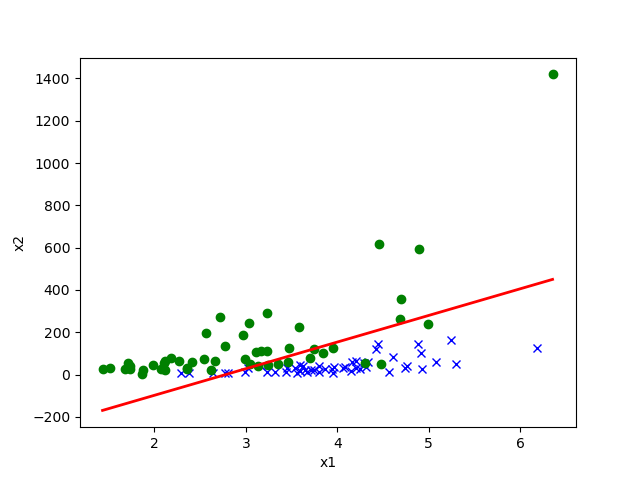
\includegraphics[width=\linewidth]{p01b_pred_1_txt.png}
        \subcaption{Logistic Regression for Dataset 1}
    \end{subfigure}
    \begin{subfigure}[b]{0.5\linewidth}
        \centering
        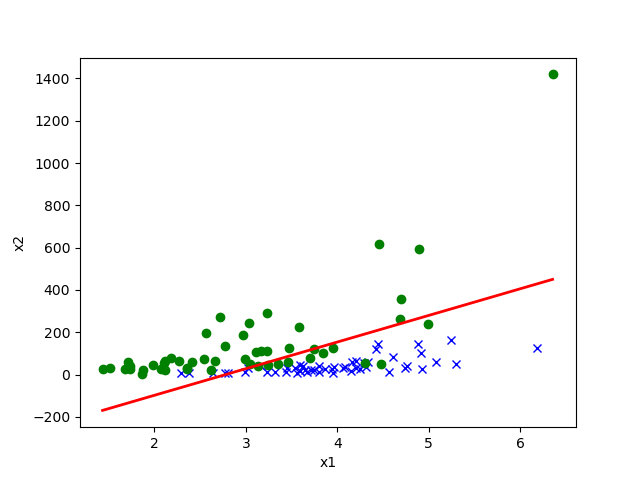
\includegraphics[width=\linewidth]{p01e_pred_1_txt.png}
        \subcaption{GDA for Dataset 1}
    \end{subfigure}

\end{figure}

\end{answer}
} \fi

	\clearpage
\item \subquestionpoints{5}
Repeat the steps in part (f) for Dataset 2. On which dataset does GDA seem to
perform worse than logistic regression? Why might this be the case?

\ifnum\solutions=1{
  \begin{answer}
\begin{figure}[htbp]
    \begin{subfigure}[b]{0.5\linewidth}
        \centering
        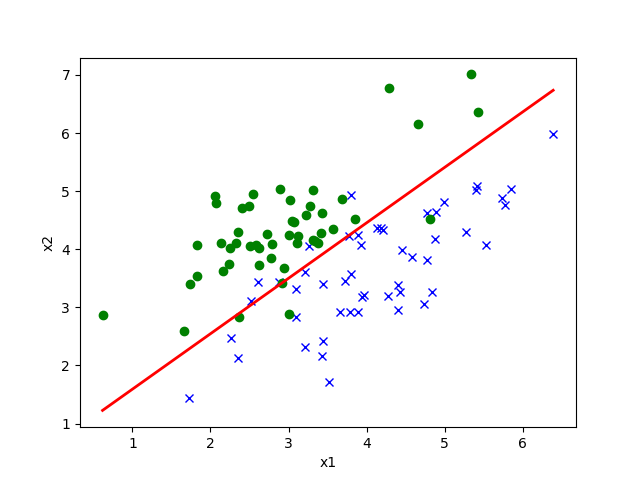
\includegraphics[width=\linewidth]{output/p01b_pred_2.txt.png}
        \subcaption{Logistic Regression for Dataset 2}
    \end{subfigure}
    \begin{subfigure}[b]{0.5\linewidth}
        \centering
        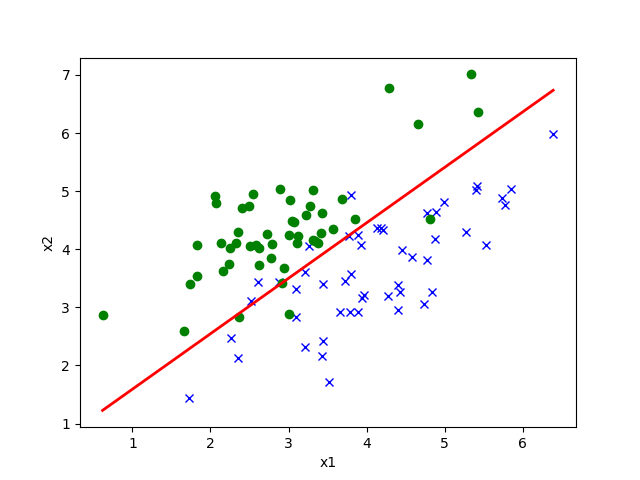
\includegraphics[width=\linewidth]{output/p01e_pred_2.txt.png}
        \subcaption{GDA for Dataset 2}
    \end{subfigure}

\end{figure}
\end{answer}

}\fi

	\clearpage
\item \points{3 extra credit} For the dataset where GDA performed worse in
parts (f) and (g), can you find a transformation of the $x^{(i)}$'s such
that GDA performs significantly better? What is this transformation?

\ifnum\solutions=1{
  \begin{answer}
\end{answer}

}\fi

\end{enumerate}


\clearpage
\item \points{40} {\bf Linear Classifiers (logistic regression and GDA)}

In this problem, we cover two probabilistic linear classifiers we have
covered in class so far. First, a discriminative linear classifier: logistic
regression. Second, a generative linear classifier: Gaussian discriminant
analysis (GDA). Both the algorithms find a linear decision boundary that
separates the data into two classes, but make different assumptions. Our goal
in this problem is to get a deeper understanding of the similarities and
differences (and, strengths and weaknesses) of these two algorithms.

For this problem, we will consider two datasets, provided in the following
files:
\begin{enumerate}[label=\roman*.]
	\item \url{data/ds1_{train,valid}.csv}
	\item \url{data/ds2_{train,valid}.csv}
\end{enumerate}
Each file contains $m$ examples, one example $(x^{(i)}, y^{(i)})$ per row.
In particular, the $i$-th row contains columns $x^{(i)}_0\in\Re$,
$x^{(i)}_1\in\Re$, and $y^{(i)}\in\{0, 1\}$. In the subproblems that follow, we
will investigate using logistic regression and Gaussian discriminant analysis
(GDA) to perform binary classification on these two datasets.

\begin{enumerate}
	\item \subquestionpoints{10}
In lecture we saw the average empirical loss for logistic regression:
\begin{equation*}
	J(\theta)
	= -\frac{1}{m} \sum_{i=1}^m y^{(i)}\log(h_{\theta}(x^{(i)}))
		+  (1 - y^{(i)})\log(1 - h_{\theta}(x^{(i)})),
\end{equation*}
where $y^{(i)} \in \{0, 1\}$, $h_\theta(x) = g(\theta^T x)$ and
$g(z) = 1 / (1 + e^{-z})$.

Find the Hessian $H$ of this function, and show that for any vector $z$, it
holds true that
%
\begin{equation*}
    z^T H z \ge 0.
\end{equation*}
%
{\bf Hint:} You may want to start by showing that
$\sum_i\sum_j z_i x_i x_j z_j = (x^Tz)^2 \geq 0$. Recall also that
$g'(z) = g(z)(1-g(z))$.

{\bf Remark:} This is one of the standard ways of showing that the matrix $H$
is positive semi-definite, written ``$H \succeq 0$.''  This implies that $J$ is
convex, and has no local minima other than the global one. If you have some
other way of showing $H \succeq 0$, you're also welcome to use your method
instead of the one above.

\ifnum\solutions=1 {
  \begin{answer}
Throughout the problem set $(a,b)$ denoted the inner(dot) product of the vectors $a,b.$
It is easy to see that for the logistic function $g(z)$, we have $g'(z)= g(z)(1- g(z)).$ We use this to calculate the partial derivative of the loss functions. 
$$\frac{\partial h_{\theta}(x)}{\partial \theta_i} = \frac{\partial g(\theta^Tx)}{\partial \theta_i} = g(\theta^Tx) (1 - g(\theta^Tx))
\frac{\partial}{\partial\theta_i}(\theta^Tx) = h_{\theta}(x) (1 - h_{\theta}(x)) x_i$$
Hence,

$$\frac{\partial log(h_{\theta}(x))}{\partial \theta_i} = \frac{h'_{\theta}(x)}{h_{\theta}(x)} = (1 - h_{\theta}(x))x_i.$$
Similarly,

$$\frac{\partial (1 - log(1 - h_{\theta}(x)))}{\partial \theta_i} = - \frac{h'_{\theta}(x)}{1 - h_{\theta}(x)} = -h_{\theta}(x)x_i.$$

Using the above computations and some simplification we obtain the partial derivative of the loss function wrt $i-$th component.
$$\frac{\partial J(\theta)}{\partial \theta_i} = - \frac{1}{m}\sum_{k = 1}^{m }x_i^{(k)}( y^{(k)} - h_{\theta}(x^{(k)})). \eqno(1)$$

Note that the above sum can conveniently be expressed in the form of inner product and we will use such form in the coding part using numpy's dot operation.

The formula (1)  allow us to easily find the entries of the Hessian.

$$\frac{\partial^2 J(\theta)}{\partial \theta_i \partial\theta_j} = 
\frac{1}{m}\sum_{k = 0}^{m - 1}g'(\theta^Tx^{(k)}))x_i^{(k)}x_j^{(k)}. \eqno(2)$$
Thus, the $(i,j)-$ th entry  of the Hessian matrix is given by the right hand side of (2).
Now we show that the Hessian is positive semi-definite. Below $(a,b)$ denotes the inner product of $a$ and $b.$
$$z^THz = (Hz,z)=  \sum_{i,j}\sum_{k = 1}^{m}g'(\theta^Tx^{(k)})x_i^{(k)}x_j^{(k)}z_iz_j=  \sum_{k = 1}^m\sum_{i,j}g'(\theta^Tx^{(k)})x_i^{(k)}x_j^{(k)}z_iz_j$$
$$= \sum_{k = 1}^m g'(\theta^Tx^{(k)}) (x^Tz)^2 \ge 0.$$
as the logistic function is non -decreasing so its derivative is non-negative (or $g' = g(1-g)\ge 0$).

\end{answer}

  
} \fi

	\clearpage
\item \subquestionpoints{5} \textbf{Coding problem.}
Follow the instructions in \texttt{src/p01b\_logreg.py} to train a
logistic regression classifier using Newton's Method.
Starting with $\theta = \vec{0}$, run Newton's Method until the updates to
$\theta$ are small: Specifically,  train until the first iteration $k$ such
that $\|\theta_{k} - \theta_{k-1}\|_1 < \epsilon$, where
$\epsilon = 1\times 10^{-5}$. Make sure to write your model's predictions to
the file specified in the code.

\ifnum\solutions=1 {
  \begin{answer}
Done!
\end{answer}

} \fi

	\clearpage
\item \subquestionpoints{5}
Recall that in GDA we model the joint distribution of $(x, y)$ by the following
equations:
%
\begin{eqnarray*}
	p(y) &=& \begin{cases}
	\phi & \mbox{if~} y = 1 \\
	1 - \phi & \mbox{if~} y = 0 \end{cases} \\
	p(x | y=0) &=& \frac{1}{(2\pi)^{n/2} |\Sigma|^{1/2}}
		\exp\left(-\frac{1}{2}(x-\mu_{0})^T \Sigma^{-1} (x-\mu_{0})\right) \\
	p(x | y=1) &=& \frac{1}{(2\pi)^{n/2} |\Sigma|^{1/2}}
		\exp\left(-\frac{1}{2}(x-\mu_1)^T \Sigma^{-1} (x-\mu_1) \right),
\end{eqnarray*}
%
where $\phi$, $\mu_0$, $\mu_1$, and $\Sigma$ are the parameters of our model.

Suppose we have already fit $\phi$, $\mu_0$, $\mu_1$, and $\Sigma$, and now
want to predict $y$ given a new point $x$. To show that GDA results in a
classifier that has a linear decision boundary, show the posterior distribution
can be written as
%
\begin{equation*}
	p(y = 1\mid x; \phi, \mu_0, \mu_1, \Sigma)
	= \frac{1}{1 + \exp(-(\theta^T x + \theta_0))},
\end{equation*}
%
where $\theta\in\Re^n$ and $\theta_{0}\in\Re$ are appropriate functions of
$\phi$, $\Sigma$, $\mu_0$, and $\mu_1$.

\ifnum\solutions=1{
  \begin{answer}
Apply Bayes
$$p(y = 1| x) = \frac{p(x| y=1)p(y = 1)}{p(x| y=1)p(y = 1) + p(x| y=0)p(y = 0)} = \frac{1}{1 + \frac{p(x| y=0)p(y = 0)}{p(x| y=1)p(y = 1)}}.$$
Note that $\frac{p(y = 0)}{p(y = 1)} = exp(ln(\frac{1-\phi}{\phi})$
For simplicity  denote A = $\Sigma^{-1}.$
Note that
$$\frac{p(x| y=0)}{p(x| y=1)} = exp(-\frac{1}{2}(A(x- \mu_0), x - \mu_0) - (A(x- \mu_1), x - \mu_1))) $$$$= exp(-\frac 12((Ax,x) - 2(Ax, \mu_0) + (\mu_0, \mu_0) - (Ax,x) + 2(Ax, \mu_1) + (\mu_1, \mu_1)))$$
$$= exp(-( -(Ax, \mu_0) + \frac 12(A\mu_0, \mu_0) + (Ax, \mu_1) - \frac12(A\mu_1, \mu_1))) = exp(-(\mu_1 - \mu_0)^TAx + \frac{1}{2}((A\mu_0,\mu_0) - (A\mu_1,\mu_1)).$$
From this we find $\theta^T = (\mu_1 - \mu_0)^TA$ hence 
$$\theta = (\Sigma^{-1})^T(\mu_1 - \mu_0)$$
and
$$\theta_0 = \frac{1}{2}((\Sigma^{-1}\mu_0,\mu_0) - (\Sigma^{-1}\mu_1,\mu_1)) - ln(\frac{1-\phi}{\phi}).$$

\end{answer}

}\fi

	\clearpage
\item \subquestionpoints{7} For this part of the problem only, you may
  assume $n$ (the dimension of $x$) is 1, so that $\Sigma = [\sigma^2]$ is
  just a real number, and likewise the determinant of $\Sigma$ is given by
  $|\Sigma| = \sigma^2$.  Given the dataset, we claim that the maximum
  likelihood estimates of the parameters are given by
  \begin{eqnarray*}
    \phi &=& \frac{1}{m} \sum_{i=1}^m 1\{y^{(i)} = 1\} \\
\mu_{0} &=& \frac{\sum_{i=1}^m 1\{y^{(i)} = {0}\} x^{(i)}}{\sum_{i=1}^m
1\{y^{(i)} = {0}\}} \\
\mu_1 &=& \frac{\sum_{i=1}^m 1\{y^{(i)} = 1\} x^{(i)}}{\sum_{i=1}^m 1\{y^{(i)}
= 1\}} \\
\Sigma &=& \frac{1}{m} \sum_{i=1}^m (x^{(i)} - \mu_{y^{(i)}}) (x^{(i)} -
\mu_{y^{(i)}})^T
  \end{eqnarray*}
  The log-likelihood of the data is
  \begin{eqnarray*}
\ell(\phi, \mu_{0}, \mu_1, \Sigma) &=& \log \prod_{i=1}^m p(x^{(i)} , y^{(i)};
\phi, \mu_{0}, \mu_1, \Sigma) \\
&=& \log \prod_{i=1}^m p(x^{(i)} | y^{(i)}; \mu_{0}, \mu_1, \Sigma) p(y^{(i)};
\phi).
  \end{eqnarray*}
By maximizing $\ell$ with respect to the four parameters,
prove that the maximum likelihood estimates of $\phi$, $\mu_{0}, \mu_1$, and
$\Sigma$ are indeed as given in the formulas above.  (You may assume that there
is at least one positive and one negative example, so that the denominators in
the definitions of $\mu_{0}$ and $\mu_1$ above are non-zero.)

\ifnum\solutions=1 {
  \begin{answer}
The product and the sums run from  1 to m, so for simplicity I drop the limits. Note that
$$l = \log\prod p(y^{(i)}| x^{(i)})p(y{(i)}) = \sum\log p(y^{(i)}| x^{(i)})p(y{(i)}) = $$$$
 -m\log(\sigma) + c_0 - \sum\big( y^{(i)}\frac{(x^{(i)} - \mu_0)^2}{2\sigma^2} + (1- y^{(i)})\frac{(x^{(i)} - \mu_1)^2}{2\sigma^2}\big) + \sum(y^{(i)}\phi + (1-y^{(i)})(1-\phi)).$$
 
 Now we calculate the partial derivatives.
 
 $$\frac{\partial}{\partial\phi} = \sum(\frac{y^{(i)}}{\phi} + \frac{1- y^{(i)}}{1-\phi}) = 0.$$
 The numerator after the sum is then $\sum y^{(i)} - m\phi$ and so
 $$\phi= \frac{\sum y^{(i)}}{m}.$$
 Not that the formula is exactly as the formula given in the problem because if $y^{(i)} = 0$ the $i-$th term of the sum is $0.$ Hence this formula can be represented with the characteristic function. I will not be re-writing this as well as the problems below as I do not know how useful it may be in the coding part.
 Further derivatives (enough to show $\mu_0$):
 $$\frac{\partial l}{\partial\mu_0} =\sum\frac{y^{(i)}(x^{(i)} - \mu_0 )}{\sigma^2} = \frac{\sum x^{(i)}y^{(i)} - \mu_0\sum y^{(i)}}{\sigma^2}.$$
 Hence we obtain
 $$\mu_0 = \frac{\sum x^{(i)}y^{(i)}}{\sum y^{(i)}}.$$
 Finally, 
 $$\frac{\partial l}{\partial \sigma} = \frac{m}{\sigma} - \frac{1}{\sigma^3}(\sum\big( y^{(i)}\frac{(x^{(i)} - \mu_0)^2}{2\sigma^2} + (1- y^{(i)})\frac{(x^{(i)} - \mu_1)^2}{2\sigma^2}\big)).$$
 By solving this equation for $\sigma$ we obtain the desired result.
 
 
 
\end{answer}

} \fi

	\clearpage
\item \subquestionpoints{3} \textbf{Coding problem.}
In \texttt{src/p01e\_gda.py}, fill in the code to
calculate $\phi$, $\mu_{0}$, $\mu_{1}$, and $\Sigma$, use these parameters
to derive $\theta$, and use the resulting GDA model to make predictions on the
validation set.

\ifnum\solutions=1 {
  \begin{answer}
\end{answer}

} \fi

	\clearpage
\item \subquestionpoints{5}
For Dataset 1, create a plot of the validation set with $x_1$ on the horizontal
axis, and $x_2$ on the vertical axis. To visualize the two classes, use a
different symbol for examples $x^{(i)}$ with $y^{(i)} = 0$ than for those with
$y^{(i)} = 1$. On the same figure, plot the decision boundary found by logistic
regression in part (b). Make an identical plot with the decision boundary found
by GDA in part (e).

\ifnum\solutions=1 {
  
\begin{answer}
\begin{figure}[htbp]
    \begin{subfigure}[b]{0.5\linewidth}
        \centering
        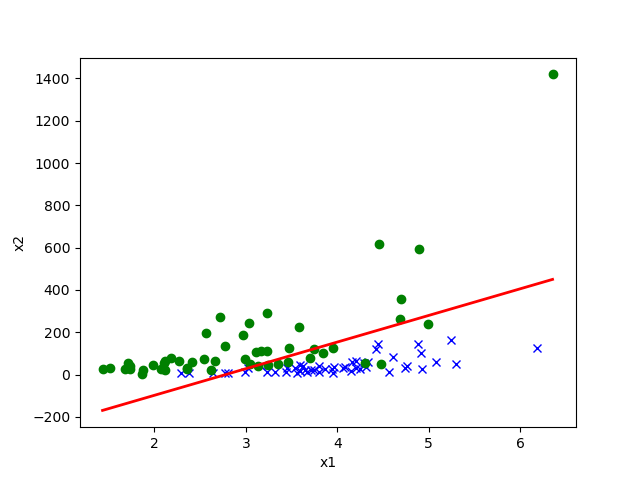
\includegraphics[width=\linewidth]{p01b_pred_1_txt.png}
        \subcaption{Logistic Regression for Dataset 1}
    \end{subfigure}
    \begin{subfigure}[b]{0.5\linewidth}
        \centering
        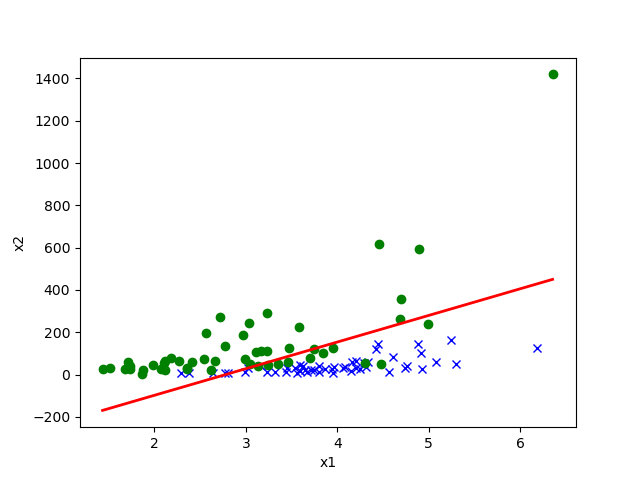
\includegraphics[width=\linewidth]{p01e_pred_1_txt.png}
        \subcaption{GDA for Dataset 1}
    \end{subfigure}

\end{figure}

\end{answer}
} \fi

	\clearpage
\item \subquestionpoints{5}
Repeat the steps in part (f) for Dataset 2. On which dataset does GDA seem to
perform worse than logistic regression? Why might this be the case?

\ifnum\solutions=1{
  \begin{answer}
\begin{figure}[htbp]
    \begin{subfigure}[b]{0.5\linewidth}
        \centering
        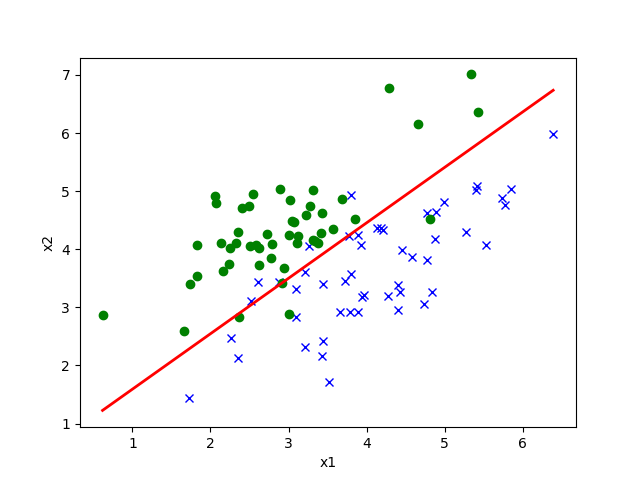
\includegraphics[width=\linewidth]{output/p01b_pred_2.txt.png}
        \subcaption{Logistic Regression for Dataset 2}
    \end{subfigure}
    \begin{subfigure}[b]{0.5\linewidth}
        \centering
        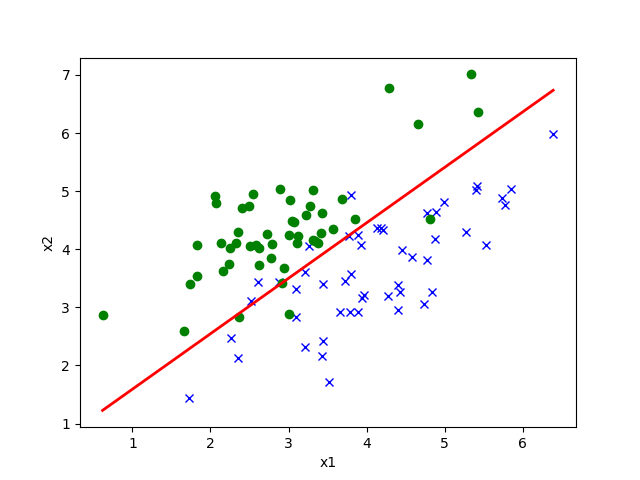
\includegraphics[width=\linewidth]{output/p01e_pred_2.txt.png}
        \subcaption{GDA for Dataset 2}
    \end{subfigure}

\end{figure}
\end{answer}

}\fi

	\clearpage
\item \points{3 extra credit} For the dataset where GDA performed worse in
parts (f) and (g), can you find a transformation of the $x^{(i)}$'s such
that GDA performs significantly better? What is this transformation?

\ifnum\solutions=1{
  \begin{answer}
\end{answer}

}\fi

\end{enumerate}


\end{enumerate}

\end{document}
